\documentclass[a4paper,12pt,oneside]{book}
\usepackage[english]{babel} 
%\usepackage[italian]{babel} 
%\usepackage[latin1]{inputenc} 
\usepackage[dvips]{graphicx}
\usepackage{amssymb}
\usepackage[width=125mm]{caption}
\usepackage{amsthm}
\usepackage[ND,SEQ]{prftree}
\usepackage{mathrsfs}
\usepackage{graphicx}
\usepackage{amsmath}


\usepackage{fancyhdr}
 
\pagestyle{fancy}
\fancyhf{}
%\fancyhead[CE]{\leftmark}
\fancyhead[CO]{\rightmark}
\fancyfoot[CE,CO]{\thepage} 
\renewcommand{\headrulewidth}{1pt}
%\renewcommand{\footrulewidth}{1pt}   %not visible if commented 

\usepackage[pdfauthor={Paolo Comensoli},
pdftitle={Applications of hyper-resolution, 
Paolo Comensoli}, pagebackref=false,bookmarksopen=true]{hyperref}
% pagebackref: se vero, ad ogni voce di bibliografia aggiunge il numero della pagine in cui viene citata
% bookmarksopen: se  vero, il pdf mostra il menu' dei contenuti gia' esploso


% Dimensione della pagina
\setlength{\oddsidemargin}{.3in}  % Distance from the left edge -1 inch 
\setlength{\textwidth}{145mm}     % Normal width of the text
\setlength{\topmargin}{.25in}     % Distance from top to PAGE'S HEAD -1 inch
\setlength{\textheight}{225mm}    % Height of the body of page
\setlength{\headheight}{0mm}      % Height of a box containing the head
\setlength{\parskip}{1mm}         % Extra vertical space before a paragraph
\setlength{\parindent}{9mm}       % Width of the indentation 
\linespread{1.65}                 % Line spacing        





\newtheorem{theorem}{Theorem}[chapter]
\newtheorem{proposition}[theorem]{Proposition}
\newtheorem{definition}[theorem]{Definition}
\newtheorem{lemma}[theorem]{Lemma}
\newtheorem{corollary}[theorem]{Corollary}
\newtheorem{example}[theorem]{Example}
\newtheorem{conjecture}[theorem]{Conjecture}


\newcommand{\E}{\mathscr{E}}
\newcommand{\D}{\mathscr{D}}

%\newcommand*{\QEDF}{\hfill\ensuremath{\blacksquare}}
\newcommand*{\QED}{\hfill\ensuremath{\square}}
\newcommand*{\QEDn}{\newline\hspace*{1cm}\QED} %quadratino nella lina sottostante


\newcommand*\npred{\,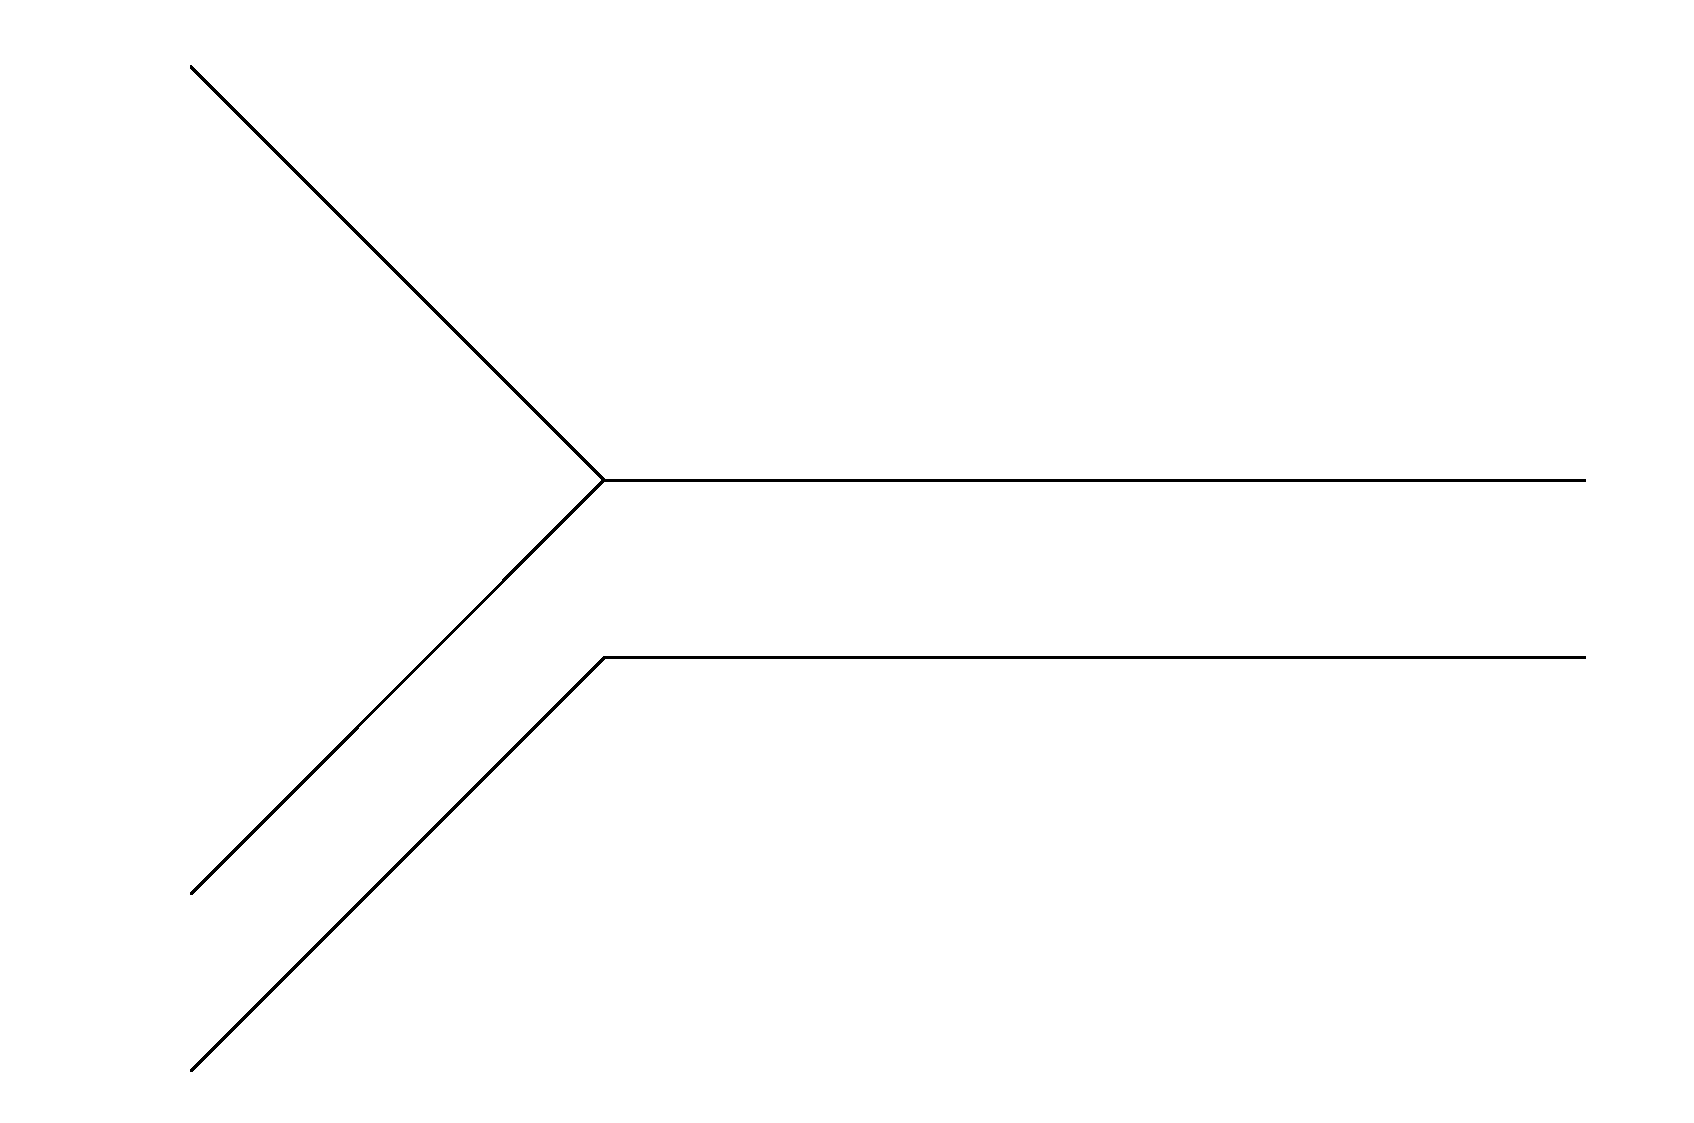
\includegraphics[scale=0.023]{./simboli/not-predecessor.eps}\,}
\newcommand*\pred{\,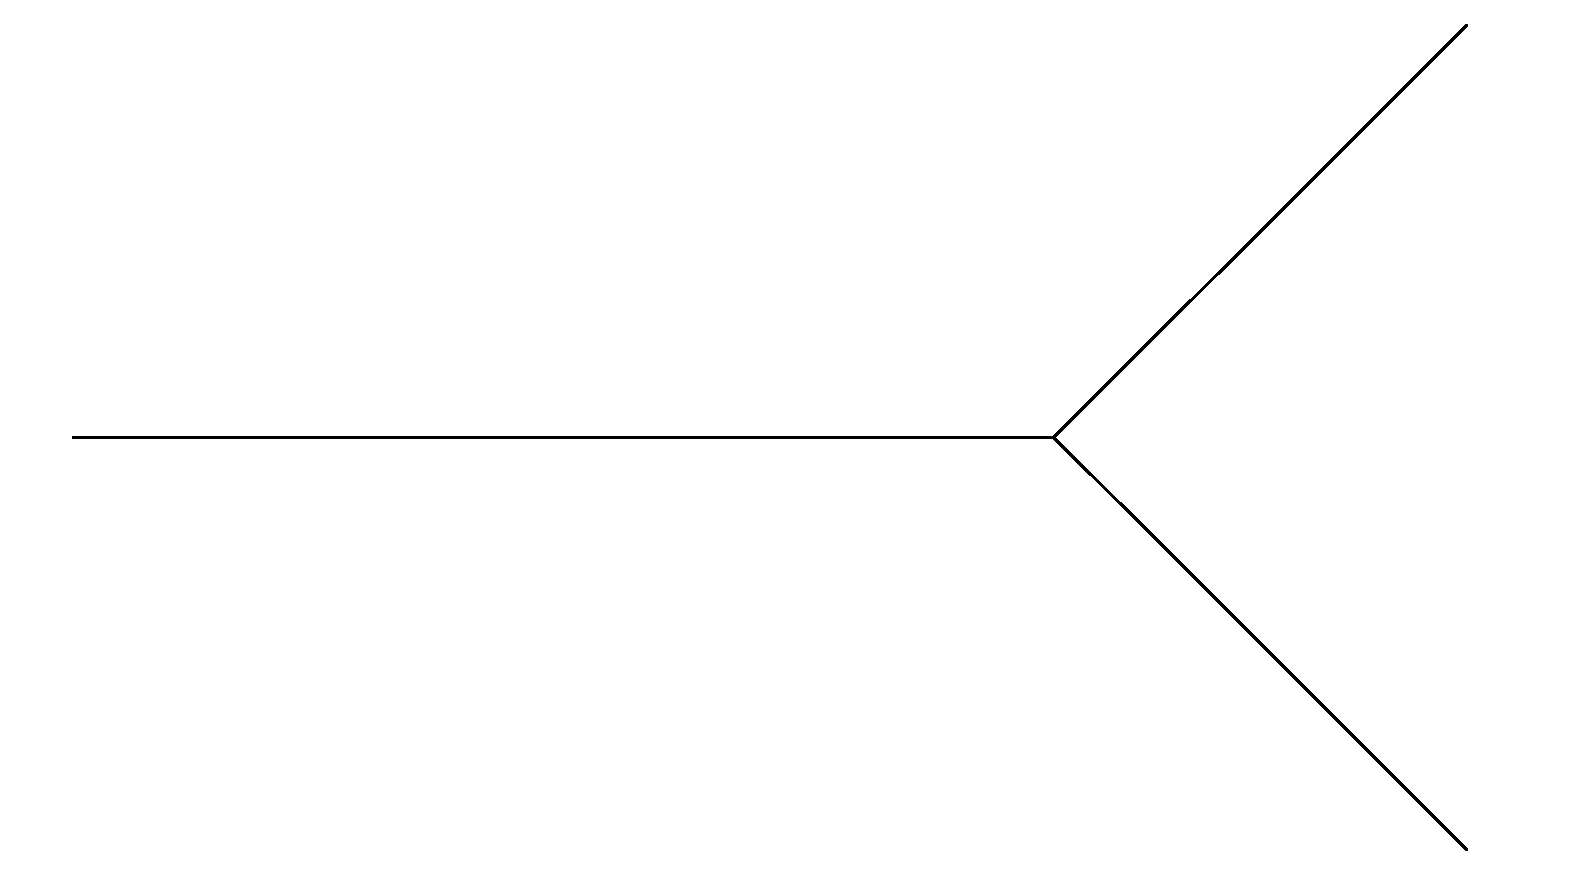
\includegraphics[scale=0.023]{./simboli/predecessor.eps}\,}



\let\oldemptyset\emptyset
\let\emptyset\varnothing
\let\o\vee
\let\e\wedge
\let\bottom\perp

\title{Applications of hyper-resolution}
\author{Paolo Comensoli}
\date{19/10/2018}

\begin{document}
 
{
\thispagestyle{empty}

\begin{center}
{\Large \textbf{Universit\`a degli studi di Verona\\}}
{\Large  Laurea Magistrale in Mathematics}
\end{center}

\vskip5cm


\begin{center}
{\huge \textbf{Applications of hyper-resolution}}
%{\small{version of \today}}
\end{center}


{\large
\vskip2.5cm\noindent Relatore:  Prof. Peter Micheal Schuster\\
Correlatore: Prof. Giuseppe Mazzuoccolo\\
Correlatore: Dott. Daniel Wessel\\
}

\vskip3cm
\hskip9cm\parbox[t]{7cm}
{\large 
Paolo Comensoli\\
Matricola n$^\circ$ VR$407226$\\
A.A. $2017$/$2018$\\
%\vskip 0.5mm Codice PACS: ?9.?a.?Z
}

\newpage
\newpage
\thispagestyle{empty}
\clearpage
}


%{
\thispagestyle{empty}


\vspace*{3cm}
%\hskip6cm\parbox[t]{9cm}
%{\large 
%\textit{"To those who err in seeking answers\\
%and have the courage to say 'we erred'\\
%Therefore, also to my parents "\\ }
%}
\hskip5cm\parbox[t]{10cm}
{\large 
\textit{"A quelli che sbagliano cercando risposte\\
e hanno il coraggio di dire 'abbiamo sbagliato'\\
Perci\`o anche ai miei genitori"\\ }
}

\vspace*{0.05cm}
\hskip12cm\parbox[t]{5cm}{\small{H. Fleischner}}


\newpage
\newpage
\thispagestyle{empty}
\clearpage
}




%----------------------------------Page of table of contents

\setlength{\parskip}{-0.7mm} 
\pdfbookmark{\contentsname}{Contents}
\setcounter{page}{1}
\tableofcontents
\thispagestyle{empty}
\newpage
\setlength{\parskip}{1mm} 



\chapter*{Introduction} %--------------------------------- CAPITOLO 1
\addcontentsline{toc}{chapter}{Introduction}
\markboth{Introduction}{Introduction}

In 1972 Matiyasevich published an article titled \textit{Application of the methods of the theory of logical derivation to graph theory} \cite{mat-2}, in which the author successfully applies proof theoretic tools to graph theory, a field of mathematics that can appear quite far from logic. 
In that paper Matiyasevich  gives an inductive definition of "a graph which cannot be colored with $n$ colors." and uses it to formulate  Hadwiger's conjecture and the four colour theorem. 
Such formulations are said by  Matiyasevich to be "useful in investigation of the above hypotheses" \cite{mat-2}; this may be one of the reasons that made him publish, in 1974 and 1975, two further papers \cite{mat-3,mat-1} on the argument.
 In those articles he generalizes his approach, and finds new applications such as Vitaver's theorem on coloring of directed graphs.

The main proof theoretic tool used by Matiyasevich is the hyper-resolution calculus, which was developed by Robinson in 1965 \cite{robinson,rob,robinson-general}. 
In the paper \textit{A Machine-oriented logic based on the resolution principle} \cite{robinson} Robinson defines the \textit{resolution principle}, a single inference principle which provides, by itself, a complete system of propositional calculus.  
In the following papers  \cite{rob,robinson-general}, he generalizes the resolution principle to hyper-resolution principle. 
The main advantage of the latter  is that, while deduction trees in resolution calculus are binary, the trees in hyper-resolution calculus can branch more  and deductions are more compact.


\newpage\vspace*{1mm}
In 1980 Lifschitz, starting from Matiyasevich's work, applied hyper-resolution to algebra \cite{lifschitz}; in particular he proved Hilbert's Nullstellensatz using Robinson's completeness theorem of hyper-resolution calculus. 
To achieve that proof, Lifschitz elaborated four equivalent versions of the completeness theorem; the last one is formulated in such a way that can be readily applied to many kinds of problems.

In this work we will see several applications of the hyper-resolution calculus to fields of mathematics different from proof theory. 
In the first chapter, we will give a definition of the hyper-resolution calculus; since we are interested in applications, we will take in particular account Lifschitz's versions of the completeness theorem. The second Chapter is dedicated to algebraic applications; the main goal is to see how the tools developed in chapter 1 can be applied to commutative algebra. To that aim, first we will see how it is possible to represent vector spaces and fields using hyper-resolutions, then we will use such knowledge to prove the Nullstellensatz. 

In the last chapter we will see several applications to graph theory. We will focus on coloring problems, and we will see two different ways to describe a coloring map using hyper-resolution. We will move from 
Matiyasevich's work \cite{mat-2,mat-3,mat-1}, and we will see his results using Lifschitz's versions of the completeness theorem.  We prefer to use Lifschitz's approach since it is more direct and clear than Matiyasevich's original one. 



\chapter{Hyper-resolution}
In 1965, Robinson presented a propositional logic which is specifically designed for use as theoretical instrument of a computer theorem-proving program \cite{robinson}. A prominent feature of this logic system is that it is based on one single inference principle, the resolution principle. 
The formalism is based upon the notions of unsatisfiability and refutation rather than upon validity and proof. The resolution technique uses proof by contradiction, and is based on the fact that any formula in propositional logic can be transformed into an equivalent formula in conjunctive normal form. 
The main perk of resolution principle is its ability to avoid the major combinatorial obstacles in the theorem proving procedures  \cite{robinson}.
The hyper-resolution principle is a natural generalization which was formulated by Robinson \cite{rob,robinson-general} few months after the resolution principle. Starting from this principle and from Matiyasevich's work \cite{mat-1}, Lifschitz \cite{lifschitz} developed a way to apply the hyper-resolution principle to parts of mathematics other than proof theory.

\newpage
\section{Preliminaries}
The aim of this section is to introduce the resolution calculus. First of all we introduce some elements which are necessary to define the trees of this calculus; secondly we state the resolution principle. We take for granted some basic notions such as terms, relation symbols and atomic formulae. 
\begin{itemize}
\item A \textit{literal:} is either an atomic formula, or has the form $\neg A$ where $\neg$ is the negation symbol and $A$ is an atomic formula. The literals $A,\,\neg A$ are \textit{complementary}, and each is the \textit{complement} of the other. Literals will be denoted using capital Latin letters $A,B,C,...$.
\item A \textit{clause:} is a finite set of literals. Clauses are denoted by Greek capital letters $\Gamma,\Sigma ,\Pi,...$. The singleton $\{A\}$ is denoted by its element $A$, so that $\Gamma\cup A$ stands for $\Gamma\cup\{A\}$.
\item if $\Gamma$ is a clause, $\overline{\Gamma}$ is the disjunction of the elements of $\Gamma$ in a fixed order.
\item A \textit{tree of clauses} is a tree to each node of which is attached a clause. The leafs are called \textit{assumptions of the tree}, and the root \textit{conclusion of the tree}.
\end{itemize}

\begin{definition}[resolvent]
Let $\Gamma_1$ and $\Gamma_2$ be two clauses, if there is a literal $P$ such that $P\in\Gamma_1$ and $\neg P\in\Gamma_2$; then $\Pi =\Gamma_1\cup\Gamma_2\setminus\{P,\neg P\}$ is called the resolvent of $\Gamma_1$ and $\Gamma_2$.
\end{definition}
The \textit{\textbf{resolution principle}} can be stated as follow:
\textit{If $\Pi$ is unsatisfiable and is the resolvent of  $\Gamma_1$ and $\Gamma_2$; then  $\Gamma_1$ and $\Gamma_2$ are unsatisfiable.}
A tree of clauses is called \textit{resolution tree}, if it is binary, and each node is either a leaf or the resolvent of its two immediate predecessors.

\newpage\noindent\begin{example}
\end{example}
\begin{center}
\begin{tabular}{ccc}
$\prftree{A}{\neg A}{\emptyset}$& \hspace{4cm}&
$\prftree{\{A,P \}}{\{B, \neg P \}}{\{A,B \}}$
\end{tabular}
\end{center}
These two trees are resolution trees, both with only one application of the resolution principle. If the clauses are interpreted as disjunction of their elements, the second tree has an analog made with the rules of natural deduction 
\begin{equation*}
\prftree{\prfassumption{A\o P}}
{\prftree{\prfboundedassumption{A} }{A\o B}}
{\prftree{\prfassumption{B\o\neg P} }{\prftree{\prfboundedassumption{B} }{A\o B}}
 { \prftree{ \prftree{\prfboundedassumption{P}}{\prfboundedassumption{\neg P}}{\bottom}}{\prfassumption{ \bottom\rightarrow A\o B }}{A\o B} } 
{ A\o B} }
{A\o B}
\end{equation*}

%alternativa che richiede DNA
%\begin{equation*}
%\prfsummary{ \prftree{ \prftree{A\o B\;} {\prfboundedassumption{A} }
%{ \prftree{\prftree{\prfboundedassumption{B}}{\prftree{\prfboundedassumption{\neg B \e\neg C}}{\neg B}}{\bottom}}
%{\prfassumption{\bottom\rightarrow A}}{A} }  {A}}
%{ \prftree{\neg A\o C\;} {\prfboundedassumption{\neg A} }
%{ \prftree{\prftree{\prfboundedassumption{C}}{\prftree{\prfboundedassumption{\neg B \e\neg C}}{\neg C}}{\bottom}}
%{ \prfassumption{\bottom\rightarrow \neg A}}{\neg  A} }  {\neg A}}
%{ \prftree{\bottom} 
%{ (\neg B \e \neg C ) \rightarrow\bottom}}}
%{B\o C}
%\end{equation*}

The examples suggest that the clause shall be read as a disjunction of its elements and the empty clause as \textit{false}. Indeed we interpret the disjunction symbol $\bigvee$ as a function from truth values to truth values, which is defined for a clause $\Gamma$ as follow:
\begin{itemize}
\item $\bigvee \Gamma$ is  \textit{true} if there is $A\in\Gamma$ such that $A$ is true
\item  $\bigvee \Gamma$ is \textit{false} otherwise
\end{itemize}
Therefore $\bigvee\emptyset$ is false. We say that, if the empty set is the conclusion of some resolution tree, such tree is a \textit{refutation} of its leaves; the soundness theorem ensures that if there is a refutation for a set of clauses $S$, such set is also \textit{unsatisfiable}. Robinson's theorem \cite{robinson} give us also the completeness.
\begin{theorem}[Robinson]\label{originalRob}
If a set $S$ of clauses is unsatisfiable, then there is a refutation of $S$.
\end{theorem}

\newpage\noindent
The resolution principle is generalized by the following hyper-resolution principle:

\textit{From $\Gamma_1\cup A_1,\cdots\Gamma_m\cup A_m $ one may infer the resolvent $\Gamma_1\cup\cdots\cup\Gamma_m\cup \Sigma$, whenever $A_1\e\cdots\e A_m\rightarrow \overline{\Sigma}$}\\  
This inference priciple gives rise to the hyper-resolution calculus, which is sound and complete \cite{rob,robinson-general}. While the proof trees made with the resolution principle are binary, any node in a hyper-resolution tree can have any number of predecessors.


\section{Lifschitz's versions}
Matiyasevich was presumably the first to see that the hyper-resolution calculus and Robinson's theorem on its completeness can be successfully applied to discrete mathematics \cite{mat-1,mat-2}. Lifschitz applied Robinson's theorem to algebra \cite{lifschitz}; in order to do so  he defined the hyper-resolution calculus in a more convenient way, and he stated several versions of the completeness theorem which can be applied to many kinds of problems.

Let $T$ be a set of propositional formulae, each of the form:
\begin{equation}\label{prototipo}
\bigwedge_{i=1}^m A_i \rightarrow \bigvee_{j=1}^n B_j 
\end{equation}
Where the $A_i$'s and $B_j$'s are literals and $m+n>0$. For $m=0$, the formula is an axiom and will be denoted only by the disjunction $B_1\o\cdots\o B_n$. While for $n=0$, we interpret the empty disjunction as falsum, and we denote the formula by $\neg (A_1\e\cdots\e A_m)$.
Consider the following calculus $H_T$: the objects derivable are clauses and the rules of inference are:
\begin{equation}\label{axiom}
\prftree{\Gamma_1 \cup A_1 ,} {\cdots,} {\Gamma_m \cup A_m } 
{\Gamma_1\cup\cdots\cup\Gamma_m\cup\{ B_1 ,\cdots ,B_n\}}
\end{equation}
for every element of $T$. We write a derivation in $H_T$ in tree form; the leaves of the tree are called \textit{assumptions}, and the root \textit{conclusion}.


\noindent\begin{example}
\end{example} Let $T=\{ A \e B \rightarrow C \o D ,\; A,\; B,\; \neg C \}$, then $H_T$ has four rules:

\begin{center}
\begin{tabular}{cccc}
$$\prftree{\Gamma_1 \cup A } {\Gamma_2\cup B} {\Gamma_1\cup\Gamma_2\cup \{C,D\}} 
$$
& \hspace{5mm}
$$\prftree{\Gamma }  {\Gamma\cup A} 
$$
& \hspace{5mm}
$$\prftree{\Gamma }  {\Gamma\cup B} 
$$
& \hspace{5mm}
$$\prftree{\Gamma \cup C }  {\Gamma }
$$
\end{tabular}
\end{center}
Using such rules we get the tree:
$$
\prftree{\prftree{\emptyset}{A}}{\prftree{\emptyset}{B}}
{\prftree{\{C , D\}}{D}}
$$
and we write $\emptyset \vdash_{H_T} D$.  When the only assumption is the empty set, as in the example, it can be dropped and we write $\vdash_{H_T} D$.

Now Robinson's theorem \ref{originalRob} can be state as follows
\begin{theorem}[Robinson's, version 1]
If $T$ is contradictory, then $\vdash_{H_T} \emptyset$
\end{theorem}
\noindent Starting from this version, Lifschitz develops three more equivalent versions, the first one is the following
\begin{theorem}[Robinson's, version 2]\label{robinson2}
For any clauses $\Gamma_1,\cdots,\Gamma_l,\Delta$, 
if  then $\Gamma_1,\cdots ,\Gamma_l\vdash_{H_T} \Delta'$ for some $\Delta'\subseteq\Delta$
\end{theorem}

\textit{Proof}: Let $\Delta=\{C_1,\cdots,C_m\}$, and $T'= T\cup\{ \overline{\Gamma}_1, \cdots ,\overline{\Gamma}_l, \neg C_1,\cdots ,\neg C_m\}  $; then $T'$ is contradictory.
The calculus $H_{T'}$ consists of the rules of $H_T$, the axioms $\Gamma_1,\cdots\Gamma_l$ and the rules
\begin{equation}\label{negCi}
\prftree{\Gamma\cup C_i }{\Gamma }
\end{equation}
By Robinson's theorem, there exists a derivation of $\emptyset$ in $H_{T'}$. If none of the rules (\ref{negCi}) appear in such derivation, then $\Gamma_1,\cdots\Gamma_l\vdash_{H_T} \Delta'$ with $\Delta'=\emptyset$. Otherwise, consider an application of (\ref{negCi}), replace every clause $\Sigma$ that appears below it with $\Sigma\cup C_i$; the result is still a derivation in $H_{T'}$, and now the conclusion also has the literal $C_i$. Repeat this procedures until all applications of (\ref{negCi}) are eliminated, the conclusion is some subset $\Delta'$ of 	$\{C_1,\cdots,C_m\}$; the final tree uses only rules of $H_T$ or some of the axioms $\Gamma_i$, then 
$\Gamma_1,\cdots\Gamma_l\vdash_{H_T} \Delta'$
\QED


\begin{example} Let $T=\{ A ,\; \neg A \}$. Then for any $B$, $T\vdash A\rightarrow B$.
By the second version of Robinson's theorem, either $ A \vdash_{H_T} B $ or  $ A \vdash_{H_T} \emptyset$. \\Now the calculus $H_T$ has two rules:

\begin{center}
\begin{tabular}{cc}

$$\prftree{\Gamma }  {\Gamma\cup A} 
$$
& \hspace{10mm}
$$\prftree{\Gamma \cup A }  {\Gamma }
$$
\end{tabular}
\end{center}
Using this two rules, the clause $B$ is not derivable from $A$; however using the second rule we get $ A \vdash_{H_T} \emptyset$.
\end{example}
 

In the next chapters we deal with applications of hyper-resolution principle which are in first order logic, while formulae of the kind \ref{prototipo} are quantifier free. For this reason, we consider a third version of Robinson's theorem. 

\begin{theorem}[{Robinson's , version 3}] \label{Robinson3}
For any clauses $\Gamma_1, \cdots ,\Gamma_l , \Delta$, if in every model of $T$, the following is valid 
\begin{equation}\label{f_rob3}
\overline{\Gamma}_1\e\cdots\e\overline{\Gamma}_l \rightarrow \overline{\Delta}
\end{equation}
then  $\Gamma_1, \cdots ,\Gamma_l \vdash_{H_T} \Delta'$ , for some $\Delta' \subseteq \Delta$.
\end{theorem}

\textit{Proof:} If \ref{f_rob3} is valid in every model of $T$, since all the formulae in $T$ and \ref{f_rob3} are quantifier free; by completness of the propositional calculus $T\vdash (\overline{\Gamma}_1\e\cdots\e\overline{\Gamma}_l )\rightarrow\overline{\Delta}$. Then by the second version of Robinson's theorem, there is $\Delta' \subseteq \Delta$ such that $\Gamma_1, \cdots ,\Gamma_l \vdash_{H_T} \Delta'$ \QED

\newpage
\subsection*{Trivial applications}
\addcontentsline{toc}{subsection}{Trivial applications}
	
Given a rule in the form (\ref{axiom}) and an application of it in a derivation, whenever $A_i \in \Gamma_i$ for some $i$, we call such application \textit{trivial} according to Lifschitz's terminology. The following two lemmas ensure that such kind of applications can always be removed.

\begin{lemma}\label{lemma1}
Let $\Pi$ be obtained from $\Sigma_1,...,\Sigma_m$ by one application of a rule $H_T$. For any $\Sigma_1' \subseteq \Sigma_1,...,\Sigma_m' \subseteq \Sigma_m  $, one of the two following holds:\\
(a) $\Sigma_i' \subseteq \Pi$ for some $i$\\
(b) some $\Pi '\subseteq\Pi$ can be obtained from $\Sigma_1 ',...,\Sigma_m '$ by an application of the same rule
\end{lemma}

\emph{Proof:} Consider an application of (\ref{axiom}) leading from  $\Sigma_1,...,\Sigma_m$ to $\Pi$, for this application:
$$\Sigma_1=\Gamma_1\cup A_1,...,\Gamma_m\cup A_m  $$
$$\Pi=\Gamma_1\cup ...\cup\Gamma_m\cup\{B_1,...,B_n\}$$
Consider the following two cases:\\
(a) $A_i \notin \Sigma_i '$ form some $i$. Then $\Sigma_i '\subseteq\Gamma_i\subseteq\Pi$
\\(b) $A_i \in \Sigma_i '$ for every $i$. Then $\Sigma_i '=\Gamma_i ' \cup A_i$ where $\Gamma_i '=\Sigma_i '\backslash A_i $, one application of (\ref{axiom}) to 
$\Sigma_1 ',...,\Sigma_m '$ gives 
$\Pi '=\Gamma_1 '\cup ...\cup\Gamma_m '\cup\{B_1,...,B_n\}\subseteq\Pi$
\QED

\newpage
\begin{lemma}
For every derivation of a clause $\Pi$ in $H_T$ there exists a derivation of some $\Pi '\subset\Pi $ in $H_T$ without trivial application of rules of inference.
\end{lemma}

\textit{Proof:} Consider a derivation as follow
\begin{equation*}
\prftree[r]{(2)}{\prfassumption{\Sigma_1}}{\cdots}
{ \prftree[r]{(1)}{ \prfsummary{\D_1}{\Gamma_1\cup A_1} } {\cdots } { \prfsummary{\D_m}{\Gamma_m\cup A_m}} {\Sigma_k=\Gamma_1\cup\cdots\cup\Gamma_m\cup\{B_1,\cdots,B_m\}} }
{\cdots}{\prfassumption{\Sigma_l}}{\Pi}
\end{equation*}
Suppose that $(1)$ is trivial, say $A_1\in\Gamma_1$. Then $\D_1$ is a derivation of $\Gamma_1$ and we can consider the following tree

\begin{equation*}
\prftree[r]{(2')}{\prfassumption{\Sigma_1}}{\cdots}
{\prfsummary{\D_1}{\Gamma_1}}
{\cdots}{\prfassumption{\Sigma_l}}{\Pi}
\end{equation*}
Now $(2')$ is not necessarily an application of a rule of inference. However, we can apply \ref{lemma1} with  $\Sigma'_1=\Sigma_1,\cdots, \Sigma'_k=\Gamma_1\subseteq\Sigma_k\cdots\Sigma'_l=\Sigma_l$ to get either:\\
(a) $\Sigma_i' \subseteq \Pi$ for some $i$\\
(b) some $\Pi '\subseteq\Pi$ can be obtained from $\Sigma_1 ',...,\Sigma_m '$ by an application of $(2)$.\\
If it is the case of (a), the application $(2')$ is still trivial and we repeat the procedure. We keep repeating as required, the procedure terminates since at every step at least one literal is removed. \QED



\noindent This last lemma and Theorem \ref{Robinson3}  let us give a final version of Robinson's theorem.
\begin{theorem}[{Robinson's, version 4}] \label{Robinson}
For any clauses $\Gamma_1, \cdots ,\Gamma_l , \Delta$, if in every model of $T$, the following is valid 
$$
\overline{\Gamma}_1\e\cdots\e\overline{\Gamma}_l \rightarrow \overline{\Delta}
$$
then there exists a derivation of some $\Delta' \subseteq \Delta$ from $\Gamma_1, \cdots ,\Gamma_l$ in $H_T$, containing no trivial application of rules of inference.
\end{theorem}


\chapter{Applications to commutative algebra} %---------------------- CAPITOLO 2
In this chapter we show how it is possible to apply the hyper-resolution principle to commutative algebra; in particular we see how two algebraic theorems follow directly from Robinson's Theorem. Before starting with such applications, the first section briefly recalls few notions of algebra in order to fix notations and terminology, the main reference for this part is Lang's book \textit{Algebra} \cite{Lang}.
The second section presents actual applications of the hyper-resolution principle; first a  well known fact of linear algebra is proved, here we speak about vector spaces over a field, so the only operations required are addition and multiplication by a scalar. 
Second a proof of Hilbert's Nullstellensatz is presented; to do so we also need to represent the products between polynomials, so more axioms are required and the resolution calculus becomes richer.

The Nullstellensatz was first proved by Hilbert \cite{Hilbert} in 1892 , and is widely known to be a fundamental theorem for algebraic geometry. Lang, in his book,  shows Rabinowitsch's proof (1929) which is so terse that the original article \cite{Rabin} consists only of one page. 
In the second section we see the proof proposed by Lifschitz \cite{lifschitz} in 1980, this proof relies on Robinson's theorem and has two main perks; it is completely constructive, and requires a minimal algebraic background. 




\section{Basic notions of commutative algebra}
The aim of this section is to summarize few elements of algebra in order to show  Rabinowitsch's proof of  Hilbert's Nullstellensatz. All the notations and the proofs adopted here are from Lang's book \cite{Lang}. Many basic definitions, such as fields, polynomials and ideals, are not given here; indeed the main purpose is to show a classical proof of the Nullstellensatz that can be compared with Lifschitz's one.
For the same reason, many results and theorems are taken for granted, and some proofs are not given.



%Let $(A,+, \cdot)$ be a commutative ring; a subset $I$ of $A$ is an \textit{ideal} if
%\begin{itemize}
%\item[-] $(I,+)$ is a subgroup
%\item[-] from $a\in I$, $b\in A$ follows $a\cdot b\in I$ 
%\end{itemize}

For a field $K$, the ring of the polynomials with coefficients in $K$ and $n$ variables is denoted as $K[x_1,...,x_n ]$. We often use vectorial notation, letting  $x$ denote the n-tuple $(x_1,...,x_n)$ and $K[\mathbf{x}]= K[x_1,...,x_n ] $.


If $K$ is a field and $E$ an extension of it, we say that an element $x$ of $E$ is \textit{algebraic} over $K$ if there are $a_0, ..., a_n\in K$ not all zero, such that
$$ a_0 + a_1 \cdot \alpha + ...+ a_n \cdot \alpha^n=0 $$ 
which amounts to require that $\alpha$  is a zero of some polynomial with coefficients in $K$. The extension $E$ is called \textit{algebraic} if every element of $E$ is algebraic over $K$. 
Also, for $\alpha_1, ...,\alpha_n $, we denote as $K(\alpha_1, ...,\alpha_n) $ the smallest subfield of $E$ that contains $\alpha_1, ...,\alpha_n$. The field $E$ is said to be \textit{finitely generated} if for some $\alpha_1, ...,\alpha_n$, we have that $E=K(\alpha_1, ...,\alpha_n)$. 
The following lemma gives a property about rings of polynomials that is used later.
\begin{lemma}\label{finit_gen}
Let $K$ be a field and $K[\mathbf{x}]$ a finitely generated extension of it. If $K[\mathbf{x}]$ is a field then it is also algebraic over $K$
\end{lemma}

A field $K$ is called \textit{algebraically closed} if every non constant polynomial in $K[x]$ has a root in $K$. It is known that for any field $K$, there is an extension which is algebraically closed, algebraic over $K$ and unique up to isomorphism;  such extension will be called \textit{algebraic closure of $K$} and denoted as $K^a$. The algebraic closure is the maximal extension, indeed a field is algebraically closed if and only if it does not have proper algebraic extensions. 

\begin{theorem}\label{zeros}
Let $K$ be a field and $I$ an ideal in $K[x_1,...,x_n]$; then either $I=K[\mathbf{x}]$ or $I$ has a zero in $K^a$
\end{theorem}

\textit{Proof:}
Suppose $I\neq K[\mathbf{x}]$. Then there is some maximal ideal $M$ that contains $I$, and $K[\mathbf{x}]/M$ is a field. Such field is a finitely generated extension of $K$, because it is generated by $x_1, ... x_n$ mod $M$. By Lemma \ref{finit_gen} the field $K[\mathbf{x}]/M$ is algebraic over $K$ and therefore can be embedded into $K^a$ by some map $e:K[\mathbf{x}]/M \rightarrow\nobreak K^a$. Now consider the canonical map mod $M$  $\pi : K[\mathbf{x}] \rightarrow K[\mathbf{x}]/M$, then the homomorphism $h=e\circ\pi : K[\mathbf{x}]\rightarrow K^a$ gives the desired zero of $I$. \QED

Theorem \ref{zeros} implies that if a family of polynomials have a common zero in some field, then they have a common zero in the algebraic closure of $K$. 

\begin{theorem}[Hilbert's Nullstellensatz]\label{langsnulls}
Let $K$ be a field and $I$ an ideal in $K[\mathbf{x}]$, let $f$ be a polynomial of $K[\mathbf{x}]$ such that $f(c)=0$ for every zero of $I$ in $K^a$. Then there exists a natural number $p$ such that $f^p\in I$
\end{theorem}

\textit{Proof:} If $f=0$, clearly $f\in I$ since any ideal is a subgroup with respect to the addition; therefore  Let $f\neq 0$. We introduce a new variable $y$ and consider the ideal $I'$ generated by $I$ and $1-y\cdot f$. By Proposition \ref{zeros} and the current assumptions, the ideal $I'$ must be the whole polynomial ring $K[\mathbf{x},\mathbf{y}]$. In particular, 1 is in $I'$ and so for some $g_0,\cdots,g_l\in K[\mathbf{x},\mathbf{y}]$ and $f_1,..,f_l\in I$

$$ 1= g_0 \cdot (1-\mathbf{y}\cdot f) + g_1\cdot f_1 + ...+ g_l\cdot f_l  $$ 

\noindent Now let $p$ be the max degree of the polynomials $g_1,...g_l$ for the variable $y$. Then
substitute $y$ for $1/f$, and multiply both sides by  $f^p$ to clear all the denominators on the right-hand side. So by setting $h_i= f^p \cdot g_i$, we get

$$ f^p= h_1\cdot f_1 + ...+ h_l\cdot f_l   $$
that means $f^p\in I$  \QED

\noindent Later we will see a proof of this theorem that uses resolutions methods, the formulation will be slightly different as follows:

\noindent\textit{Let $K$ be a field and $f,f_1,\cdots, f_l \in K[\mathbf{x}]$, if in any extension of $K$, $f$ vanishes at all common zeros of $f_1,\cdots, f_l$, then there exists $p\in \mathbb{N}$ and $h_1,\cdots, h_l \in K[\mathbf{x}]$ such that} 
$$
f^p = \sum_{i=1}^l h_i \cdot f_i
$$

\noindent The premise of this version is equivalent of the one stated in \ref{langsnulls}, that says\\ \textit{Let $f$ be a polynomial of $K[\mathbf{x}]$ such that $f(c)=0$ for every zero of $I$ in $K^a$}.
 Indeed if $f$ vanishes at all common zeros of $f_1,\cdots, f_l$, then $f$ belongs to the ideal $I$ generated by the polynomials  $f_i$. Conversely if $f$ vanishes for every zero of $I$, this is true in particular for some generators $f_1,...,f_l$ of $I$. Also if this happens in all extensions this is true in particular for $K^a$; and if it is true for all the zeros of $K^a$ it also holds for every zeros of every extensions.


\section{Applications}
Now two concrete cases are presented; both are described by Lifschitz \cite{lifschitz} with the purpose of establishing connections between proof theory and algebra. Besides that, the following examples show how it is possible to encode algebraic items, such as vector spaces and polynomials, into a hyper-resolution calculus. Once the calculus is properly defined, the problem becomes mainly proof theoretic, and we can use Robinson's theorem.


\subsection*{Linear equations}
\addcontentsline{toc}{subsection}{Linear equations}
 
We want to give a hyper-resolution interpretation to the vector spaces over a given field $K$; consider the language with the following symbols\\
- for any $\alpha\in K$, a unary function symbol $\alpha\cdot$ for multiplication by the scalar $\alpha$\\
-  the binary function symbol +\\
- the unary relation symbol $=0$\\
Terms of this language are the linear forms of $K$, and atomic formulae are homo\-geneous linear equations. For any terms $r,s$, $r=s$ stands for $r-s=0$. Now consider the following axioms
\begin{eqnarray}
&0\cdot r =0 \\ \label{vec.spac1}
&r_1=0\rightarrow r_2 =0  \qquad (r_1,r_2 \texttt{ represent the same linear form}) \\
& ( r=0 \e s=0 )\rightarrow r+s =0 \\
& r=0 \rightarrow \alpha\cdot r =0 \label{vec.spac.ultimo}
\end{eqnarray}
These axioms imply all equality axioms and axioms of vector spaces over $K$. The models of this theory, factorized with respect to $x=y$, are precisely the vector spaces over $K$.
We will refer to the set of all possible instances of these axioms as the set $L$, which gives rise to the calculus $H_L$. 

\noindent The inference rules of $H_L$ are

\begin{equation} \label{rule1}
\prftree{\Gamma}{\Gamma\cup 0\cdot r=0 }
\end{equation}

\begin{equation} \label{rule2}
\prftree{\Gamma\cup r_1=0 }{\Gamma\cup r_2=0 }
\end{equation}

\begin{equation} \label{rule3}
\prftree{\Gamma\cup r=0} {\Delta\cup s=0 }{\Gamma\cup\Delta\cup  r+s=0}
\end{equation}

\begin{equation} \label{rule4}
\prftree{\Gamma\cup r=0}{\Gamma\cup \alpha\cdot r=0 }
\end{equation}

\noindent The following two lemmas give us information about the behavior of trees in $H_L$
\begin{lemma}\label{lemma_nempty}
The clause $\emptyset$ cannot be derived in $H_L$
\end{lemma}
\textit{Proof:} Rules (\ref{rule1}), (\ref{rule2}), (\ref{rule4}) do not reduce the number of literals involved and therefore cannot be used to deduce $\emptyset$. Rule (\ref{rule3}) reduces the number of literals by one, but it works with two non-empty premises and therefore $\emptyset$ cannot be inferred using it. \QED

\begin{lemma}\label{lemma_onlysingletons}
Consider a derivation $\Gamma_1,...,\Gamma_l \vdash_{H_L} \Delta $ without trivial applications. 
If $\Gamma_i$ is a singleton for $i=1,..,l$, then all the nodes of the derivation are singletons
\end{lemma}
\textit{Proof:} If the derivation has no trivial applications, the rule ($\ref{rule1}$) can be introduced only from $\emptyset$ which is not one of the premises $\Gamma_1,...,\Gamma_l$; therefore ($\ref{rule1}$)  does not appear. All the other rules transform singletons into a singleton, since all the premises are singletons all the other nodes of the derivations shall be singletons. \QED

\begin{proposition} 
If every solution of a system of linear equations $r_1=0,...,r_l=\nobreak 0$  is a solution of a linear equation $s=0$; then $s$ is linear combination of $r_1,...,r_l$
\end{proposition}

\textit{Proof:} Let $\Delta$ be the singleton clause $\{s=0\}$, for each equation $r_i=0$  let $\Gamma_i=\{r_i=0\}$; then 
$$ \bigwedge_{i=1}^l \Gamma_i \rightarrow \Delta $$
by Robinson's Theorem, there is a derivation in $H_T$ of some $\Delta' \subseteq\Delta$ without trivial application. By Lemma \ref{lemma_nempty} $\Delta'$ is not the empty set,  and  since $\Delta$ is a singleton , $\Delta'=\Delta$ and $ \Gamma_1,...,\Gamma_l \vdash_{H_L} \Delta  $.
Since all the premises are singletons, by Lemma \ref{lemma_onlysingletons} all the nodes are singletons. The literals in $H_L$ are linear equations and when used as premises for rules (\ref{rule2}), (\ref{rule3}), (\ref{rule4}), the conclusion is a linear combination of the premises. 
Hence $s$ is linear combination of $r_1,...,r_l$.\QED


\subsection*{Nullstellensatz} \label{null}
\addcontentsline{toc}{subsection}{Nullstellensatz}


We want to prove the Nullstellensatz as stated here:

\noindent\textit{Let $K$ be a field and $f,f_1,\cdots, f_l \in K[{x}]$, if in any extension of $K$, $f$ vanishes at all common zeros of $f_1,\cdots, f_l$, then there exists $p\in \mathbb{N}$ and $h_1,\cdots, h_l \in K[{x}]$ such that} 
$$
f^p = \sum_{i=1}^l h_i \cdot f_i
$$
We need to describe the extensions of a field and the polynomials over it. To this aim, consider the first order language $\mathscr{L}=\{+,\cdot,=\nobreak 0\}\cup\nobreak K$ where $+,\cdot$ are binary function symbols, $=0$ is a unary relation symbol and the elements of $K$ are constants; so the terms are polynomials over $K$ and the atomic formulae are algebraic equations.

\noindent Now consider the theory given by the following axioms:
\begin{eqnarray}
& 0=0  \label{ax00} \\
& \neg (1 =0) \\
& r_1=0 \rightarrow r_2 =0 \qquad (r_1,r_2 \texttt{ are equal polynomials}) \\
& ( r=0 \e s=0) \rightarrow r+s=0 \\
& r=0 \rightarrow r\cdot s=0 \\
& r\cdot s=0 \rightarrow (r=0 \o s=0) \label{axintdom}
\end{eqnarray}
One can prove the equality axioms, the axioms of integral domain and the diagram of $K$. It follows that the models of the theory are the integral domains that contain $K$. Lifschitz, instead of the axiom $\neg (1=0)$, uses the axioms  $\neg (\alpha =0)$ for each $\alpha\in K\setminus \{0\}$, however the one taken here is equivalent and simplifies the next arguments.  

Let $N$ be the set of all possible instances of the axioms; the calculus $H_N$ consists of the axiom $\{0=0\}$ and of the rules of inference:

\begin{equation}\label{non1=0}
\prftree{\Gamma \cup 1=0}{\Gamma}
\end{equation}

\begin{equation}\label{eqpoly}
\prftree{\Gamma \cup r_1=0 } { \Gamma \cup r_2=0 } \qquad r_1,r_2\texttt{ are equal polynomials}
\end{equation}

\begin{equation}\label{somm}
\prftree{\Gamma \cup r=0 \, ,}{\Delta \cup s=0}{\Gamma \cup \Delta \cup r+s=0 } 
\end{equation}

\begin{equation} \label{mol}
\prftree{\Gamma \cup r=0}{\Gamma \cup r\cdot s=0 } 
\end{equation}

\begin{equation} \label{intdom}
\prftree{\Gamma \cup r\cdot s=0}{\Gamma \cup  \{r=0,s=0\} } 
\end{equation}
Note that the rules (\ref{non1=0}-\ref{mol}) do not increase the number of elements of the clauses, precisely for an application 
$$
\prftree[r]{(\ref{non1=0}-\ref{mol}) } {\Gamma}{\Delta}{\hspace{2mm}\Sigma\hspace{2mm}}
$$
we have $ |\Sigma| \leq   |\Gamma\cup\Delta|$; while for rule (\ref{intdom})
we have $\Delta = \emptyset$ and  $ |\Sigma| =   |\Gamma| +1 $. \\

For any derivation in $H_N$ there is a tree with all the applications of the rule (\ref{intdom}) at the bottom; this is ensured by the following.
\begin{lemma}\label{lemma_nullest}\textit{Every derivation in $H_N$ which contains non-trivial applications can be rearranged in such a way that any application of (\ref{intdom}) is either the last one or it is followed by an application of (\ref{intdom})}.
\end{lemma}
\emph{\noindent \textit{Proof: }}Suppose to have a non-trivial application of a rule (\ref{intdom}) followed by a rule ($x$) different from (\ref{intdom}):
$$
\prftree[r]{$x$}
{\prftree[r]{(\ref{intdom})}
{\Gamma\cup r\cdot s=0 }
{\Gamma\cup\{r=0, s=0 \}\,,}
}
{\Delta \hspace{13mm}} 
{\hspace{7mm}\Sigma\cup\{r=0,s=0 \}\hspace{13mm}}
$$

\noindent Here $\Delta$ is the second premise in case ($x$) is the rule (\ref{somm}), otherwise it should be dropped. In the case that both $r=0$ and $s=0$ in the conclusion are different from $A_1$  shown in the scheme (\ref{axiom}) of the rule ($x$), then $A_1\in\Gamma$  and we can change the order as follows:

$$
\prftree[r]{(\ref{intdom})}
{\prftree[r]{$x$}
{\Gamma\cup r\cdot s=0 \, , \hspace{7mm}}    {\Delta \hspace{5mm}}
{\hspace{7mm}\Sigma\cup r\cdot s=0 \hspace{7mm}}}
{ {\Sigma\cup\{r=0, s=0 \}}} 
$$

\noindent Otherwise let $\{r=0\}$ be $A_1$ of ($x$), depending on whether ($x$) is (\ref{non1=0}),(\ref{eqpoly}), (\ref{somm}) or (\ref{mol}), change the derivation according to one of the schemes below


\begin{eqnarray*}
\prftree[r]{(\ref{non1=0})} { \prftree[r]{(\ref{intdom})} {\Gamma \cup  1\cdot s=0 } {\Gamma \cup  \{1=0, s=0\}} } {\Gamma \cup s=0 }
&  \leadsto 
 &\prftree[r]{(\ref{eqpoly})} { \Gamma \cup 1\cdot s=0    } {\Gamma \cup s=0}
\end{eqnarray*}



\begin{eqnarray*}
\prftree[r]{(\ref{eqpoly})} { \prftree[r]{(\ref{intdom})} {\Gamma \cup  r_1\cdot s=0} {\Gamma \cup  \{r_1=0, s=0\}} } {\Gamma \cup \{r_2=0, s=0\}}
&  \leadsto 
\prftree[r]{(\ref{intdom})} { \prftree[r]{(\ref{eqpoly})} {\Gamma \cup  r_1\cdot s=0} {\Gamma \cup  r_2\cdot s=0} } {\Gamma \cup \{r_2=0, s=0\}}
\end{eqnarray*}


\begin{eqnarray*}
\prfrulenameskip=0.4em\prflinepadbefore=1ex
\prftree[l]{(\ref{somm})} { \prftree[l]{(\ref{intdom})} { \Gamma \cup  r\cdot s=0} { \Gamma \cup \{ r=0,s=0\} }  }{ \Delta \cup t=0 }
{\hspace{11mm}\Gamma \cup \Delta \cup\{r+t=0, s=0\}\hspace{11mm}}
& \leadsto
& \prftree[r]{(\ref{intdom})} 
{\prftree[r]{(\ref{eqpoly})}
{ 
\prftree[r]{(\ref{somm})}{\Gamma \cup r\cdot s=0,} 
{ \prftree[r]{(\ref{mol})} {\Delta \cup t=0  }  {\Delta \cup t\cdot s=0 }}
{\Gamma \cup \Delta \cup r\cdot s+t\cdot s=0 }
}
{\Gamma \cup \Delta \cup (r+t)\cdot s=0 }
}
{\Gamma \cup \Delta \cup\{r+t=0, s=0\}}
\end{eqnarray*}


\begin{eqnarray*}
\prftree[r]{(\ref{mol})} { \prftree[r]{(\ref{intdom})} {\Gamma \cup  r\cdot s=0} {\Gamma \cup  \{r=0, s=0\}} } {\Gamma \cup \{r\cdot t=0, s=0\}}
&  \leadsto 
\prftree[r]{(\ref{intdom})} 
{ \prftree[r]{(\ref{eqpoly})} 
{\prftree[r]{(\ref{mol})}
{\Gamma \cup r\cdot s=0}
{\Gamma\cup (r\cdot s) \cdot t=0 } } 
{\Gamma \cup  (r\cdot t) \cdot s=0} } 
{\Gamma \cup \{r\cdot t=0, s=0\}}
\end{eqnarray*}
By a series of application of this procedure, we obtain a derivation as required. 

\QED

\begin{theorem}[Hilbert's Nullstellensatz]
Let $K$ be a field and $f,f_1,\cdots, f_l \in K[{x}]$, if in any extension of $K$, $f$ vanishes at all common zeros of $f_1,\cdots, f_l$, then there exists $p\in \mathbb{N}$ and $h_1,\cdots, h_l \in K[{x}]$ such that
$$
f^p = \sum_{i=1}^l h_i \cdot f_i
$$
\end{theorem}
\newpage
\textit{Proof: }If $f$ vanishes at all common zeros of $f_1\cdots f_l$, in every model of the axioms \ref{ax00}-\ref{axintdom} the following is valid:
$$ \Gamma_1\e\cdots\e\Gamma_l\rightarrow\Delta$$
where $\Gamma_i=\{f_i=0\}$ and $\Delta =\{f=0\}$.\\ By Robinson's theorem: $\Gamma_1,\cdots ,\Gamma_l \vdash_{H_N} \Delta '$ where either $\Delta '=\emptyset$ or $\Delta '=\{f=0\}$. 
In particular take a derivation without trivial applications and where all the applications of (\ref{intdom}) are at the bottom, the possibility of building such tree is ensured by Lemma \ref{lemma_nullest}. The tree is of the form:
\begin{equation*}
\prfsummary[only rules (\ref{intdom})] {\prftree[r]{(\ref{non1=0})-(\ref{mol})}{\Gamma_1,}{...,}{\Gamma_l}{\Sigma}}{\Delta '}
\end{equation*}
Since all the $\Gamma_i$'s are singletons, and since the rules (\ref{non1=0})-(\ref{mol}) do not increase the size of the clauses, $\Sigma$ is either a singleton or the empty set. Let's treat separately the cases of $\Delta '$.

\textbf{\emph{Case $\Delta '=\emptyset$}} \\
The only way to get $\emptyset$ out of the rules of inference is by applying (\ref{non1=0}), in this case rule (\ref{intdom}) does not apply at all, and the tree is of the form: 
$$
\prftree[r]{(\ref{non1=0})}
{ \prftree[r]{(\ref{eqpoly}) - ( \ref{mol})}
{ \Gamma_1, }{\cdots ,}{\Gamma_l}
{\hspace{5mm}\{1=0\}\hspace{5mm}	} 
}
{\emptyset }
$$
1 is obtained by a series of applications of rules (\ref{eqpoly}) - (\ref{mol}), and therefore is a linear  combination of $f_1,\cdots ,f_l\;$ : 
$$f^0=1 = \sum_{i=1}^l h_i \cdot f_i$$

\newpage

\textbf{\emph{Case $\Delta '=\{f=0\}$ }} \\
Suppose that rule (\ref{intdom}) applies $p-1$ times, (\ref{non1=0}) does not apply at all and the tree is of the form:
$$
\prftree[r]{$(p-1)$ applications of (\ref{intdom})}
{ \prftree[r]{(\ref{eqpoly}) - (\ref{mol})}
{ \Gamma_1, }{\cdots ,}{\Gamma_l}
{\hspace{7mm}\Sigma\hspace{7mm}	} 
}
{\{f=0\} }
$$
Since (\ref{intdom}) applies and $\Sigma$ is a singleton, $\Sigma$ must be of the form $ \{ t_1 \cdot r_1 =0 \}$. Suppose that the $A_1$ of the $i^{th}$ application is $r_i=t_{i+1}\cdot r_{i+1}$, then the tree is:
$$
\prfsummary{
\prftree[r]{ (\ref{intdom})}
{ \prftree[r]{(\ref{eqpoly}) - (\ref{mol})}
{ \Gamma_1, }{\cdots ,}{\Gamma_l}
{\hspace{7mm}\{t_1 \cdot r_1=0\}\hspace{7mm}	} 
}
{\{ t_1=0, t_2 \cdot r_2=0\} }
}
{\prftree[r]{(\ref{intdom})}
{\{ t_1=0,\cdots t_{p-2}=0, t_{p-1}\cdot r_{p-1}=0\}  }
{\{ t_1=0,\cdots ,t_{p-1}=0,r_{p-1}=0\}}
}
$$
Since the root of the tree must be the singleton $\Delta '=\{f=0\}$, it is the case that for any $i$: $t_i=r_{p-1}=f $.
Therefore $\Sigma= \{ f^p =0 \}$ and we conclude 
$$f^p = \sum_{i=1}^l h_i \cdot f_i $$
because  $f^p$ is obtained by a series of applications of rules (\ref{eqpoly}) - (\ref{mol}).

\QED




\chapter{Applications to graph theory}%----------------------------- CAPITOLO 3
In this chapter we discuss applications of the hyper-resolution principle to graph theory, in particular we  face two different and equivalent ways of describing $n$-colorable graphs via resolution. The first approach relies on propositions of the kind "the vertex $x$ has the same color of the vertex $y$", this method is used to give a constructive proof that a graph is 2-colorable if and only if it does not contain odd cycles. The second approach assigns to each color a number, and relies on proposition of the kind "the vertex $x$ has a color number smaller than the one of $y$", in other words this method introduces a partial order on the vertices and therefore it introduces a stronger transitivity rule. This method is used to prove the Gallai-Hasse-Roy-Vitaver theorem, which gives a characterization of the chromatic number of a simple graph, by describing a partial order among vertices using directed paths, and retrieving the $n$-colurable property by showing that such order can be used also for colors. 
Both methods are described by Matiyasevich in 1975 \cite{mat-1}; in this article Matiyasevich defines how it is possible to apply hyper-resolutions to discrete mathematics, and applies his method to coloring problems.
Last, we describe the $\mu_n$ graphs, a family of graphs introduced in 1972 by Matiyasevich \cite{mat-2}, in order to give an inductive definition of the property "a graph which cannot be colored with $n$ colors". This definition lets us generalize the characterization of bipartite (2-colorable) graphs, and lets state the four color theorem and the Hadwiger conjecture in terms of $\mu_n$ graphs.


\section{Basic notions of graph theory}

In this section we briefly recall some notions of graph theory; for the part on simple graphs we adopt the notation and terminology of Diestel \cite{diestel}, while for directed graphs the main reference is Chartrand-Zhang \cite{chrom}. Some of the results shown here are also shown in the next section using resolution methods, it might be interesting to compare the proofs and how different they are.

A simple graph $G$ is a pair of sets $(V,E)$ such that the elements of $E$ are unordered pairs of elements of $V$. The elements of $V$ are called \textit{vertices} and the elements of $E$ are called \textit{edges}. A vertex $v$ is \textit{incident} with an edge $e$ if $v$ is one of the two elements of $e$, the two vertices incident to an edge are called its \textit{ends} and are said to be \textit{adjacent}; an edge whose endpoints are $x$ and $y$ is denoted as $xy$. A graph is called  \textit{complete} if all of its vertices are pairwise adjacent; a complete graph with $n$ vertices is denoted with $K^n$.
A graph $G'=(V',E')$ is a \textit{subgraph} of G if $V' \subseteq V$ and $E' \subseteq E$.

A \textit{path} is a graph $P=(V,E)$ of the form:
$$ V=\{x_0,x_1, ..., x_n\} \qquad E=\{x_0 x_1, x_1x_2,.. x_{n-1}x_n\}$$ 
where the vertices are pairwise different, the length of the path is defined as the cardinality of $E$ which is $n$; we often refer to a path by the natural sequence of the vertices, writing $P=x_0x_1...x_n$. A graph is \textit{connected} if for any two distinct vertices, there is a path between them which is a subgraph of the given graph.  
A \textit{cycle} is a path where $x_n$ coincides with $x_0$; a cycle of length $n$ will be briefly called n-cycle; if a n-cycle is a subgraph of $G$, we say that $G$ has a n-cycle. 
 A connected graph which has no cycle is called \textit{tree}, trees are characterized by the following theorem 

\begin{theorem}[characterization of trees] The following are equivalent:
\begin{itemize}
\item[(1)] $T$ is a tree
\item[(2)] for any edge $e$ of $T$, $T-e$ is not connected   
\item[(3)] any two vertices of $T$ are linked by a unique path
\item[(4)] $T$ is maximally acyclic, i.e. for any two vertices $u,v$ such that $uv$ is not an edge of $T$, $T+uv$ has a cycle
\end{itemize}
\end{theorem}
\noindent\textit{Proof}: 

(1)$\Rightarrow$(2):\\
If $uv$ is an edge of $T$ such that $T-uv$ is still connected, there is a path from $u$ to $v$ that does not pass trough the edge $uv$, such path concatenated with $uv$ makes a cycle in $T$.

(2)$\Rightarrow$(3):\\
If there are two distinct vertices $u,v$ of $T$ which are linked by two different  paths, there is an edge $e$ which does not belong to both paths, then $T-e$ is still connected.

(3)$\Rightarrow$(1):\\
If it is connected and there is a cycle, for any two distinct vertices of the cycle there  are at least two paths linking them.

(4)$\Rightarrow$(1):\\
If it's maximally acyclic it is also connected, indeed if the vertices $u,v$ are not linked by a path, $T+uv$ would be an acyclic graph and $T$ not maximally acyclic. 

(3)$\Rightarrow$(4):\\
Let $u,v$ be two distinct vertices of $T$, such that $uv$ is not an edge of $T$, if $u,v$ are connected by a path, there is a cycle in $T+uv$, hence $T$ is maximally acyclic. \QED

 For any connected graph $G$, it is always possible to obtain a tree by only removing edges; this tree is called \textit{spanning tree} and its existence is ensured by the following constructive proof.
\begin{proposition}[Spanning Tree]
Let $G=(V,E)$ be a connected graph; then there is a tree $T=(V,E')$ such that $E'\subseteq E$
\end{proposition}
\textit{Proof:}
Consider the following procedure: If $G$ has no cycle then it is a tree and we have obtained what we were seeking; otherwise let $e$ be an edge of $G$ that belongs to a cycle, then $G-e$ is still connected and we restart the procedure with $G-e$.
The algorithm always ends since $E$ is a finite set and it returns the required tree.\QED


A \textit{k-coloring} of a graph $G=(V,E)$ is a map $c:V \rightarrow \{1,..,k\} $ such that $c(v) \neq c(w) $ whenever $v$ and $w$ are adjacent; a graph is \textit{k-colorable} if it admits a k-coloring. The minimum positive integer $k$ such that $G$ is $k-$colorable is the \textit{chromatic number} and is denoted by $\chi (G)$.

A graph $G=(V,E)$ is \textit{bipartite} if $V$ admits a partition into two subsets such that every edge has its ends in different subsets; clearly a graph is bipartite if and only if it is 2-colorable since we can assign a color to each partition to obtain a 2-coloring and conversely whenever we have a 2-coloring we immediately obtain the partitions dividing vertices according to their color. 
\begin{figure} 
\begin{center}
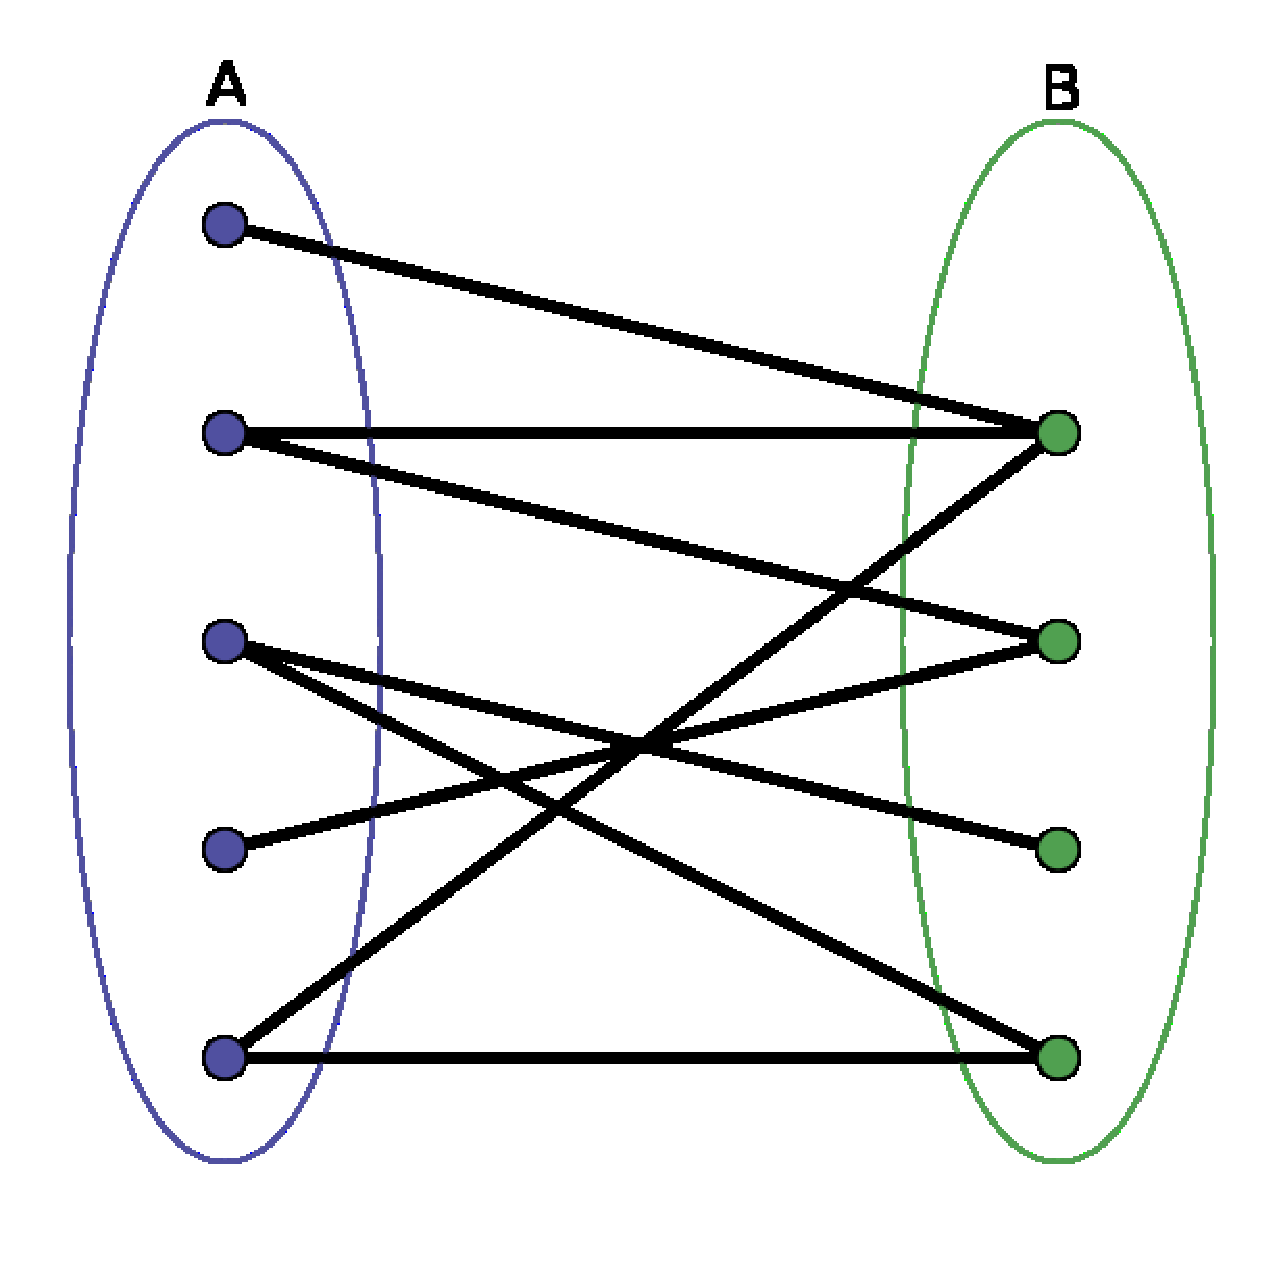
\includegraphics[scale=0.28]{bipartite.eps}
\caption{A bipartite graph colored with two colors}\label{bip}
\end{center}
\end{figure}

\newpage
Another important characterization of bipartite graphs is the property of not having cycles of odd length.
\begin{theorem}
A graph $G=(V,E)$ is bipartite if and only if it does not contain odd cycles.
\end{theorem}
\textit{Proof:}
Suppose first that $G$ is bipartite; then $V$ can be partitioned into sets $U$ and $W$, so every edge has an end in $U$ and the other in $W$. Let $C=v_1v_2...v_nv_1$ be a $n-$cycle of $G$, if we assume $v_1\in U$, then $v_2\in W$, $v_3\in U$ and so on.
In particular $v_i\in U $ when $i$ is odd and $v_i\in W$ when $i$ is even, since $v_1\in U$ it follows $v_n\in W$ and $n$ is even.

Conversely, let $G$ be a graph without odd cycles. A graph is bipartite if all its components are bipartite, so assume that $G$ is connected. Let $T=(V,E')$ be a spanning tree of $G$ and fix a vertex $r\in V$, for any $v\in V$ let $d(v)$ be the length of the unique path from $r$ to $v$; now build the partitions $U,W$ of $V$ according to the following rule:
\begin{itemize}
\item if $d(v)$ is odd, $v\in U$
\item if $d(v)$ is even, $v\in W$
\end{itemize} 
Clearly $U\cap W =\emptyset$ and $U\cup W=V$, it remains to show that any $e\in E$ has its ends in different partitions. 
Let $xy\in E$, if it is the case that $xy\in E'$ then $d(x)=d(y)\pm 1$ and therefore they belong to different partitions. If $xy\notin E'$, then adding it to the spanning tree creates a cycle $C$ which is even since it is also a cycle of $G$; thus $C-xy$ is the unique path in $T$ from $x$ to $y$ and is of odd length, whence $d(x)$ and $d(y)$ have different parity.\QED


\subsection*{Directed graphs}
\addcontentsline{toc}{subsection}{Directed graphs}

A \textit{digraph} (or directed graph) $D$  is a pair of sets $(V,A)$ where the elements of $A$ are ordered couples of $V$. Elements of $V$ are still called vertices while elements of $E$ are called \textit{arcs} or \textit{directed edges}. For instance a representation of the digraph $D=(\{x,y,z\}, \{(x,y),(y,x),(x,z),(z,y)\})$ is shown in Fig. \ref{digraph}

If for each pair of distinct vertices $u,v$ of a digraph $D$, at most one of $(u,v)$ and $(v,u)$ is an arc, $D$ is an \textit{oriented graph}. In fig. \ref{digraph} $D$ is not an oriented graph while $D_1$ and $D_2$ are good examples. Thus an oriented graph can be obtained from a simple graph $G$ by assigning a direction to each one of its edges, and the digraph obtained in this way is said to be an \textit{orientation} of $G$. On the other hand starting from an oriented graph $D$ we obtain the \textit{underlying graph } by replacing all arcs $(u,v)$ with an edge $uv$. 

\begin{figure}[h]
\centering
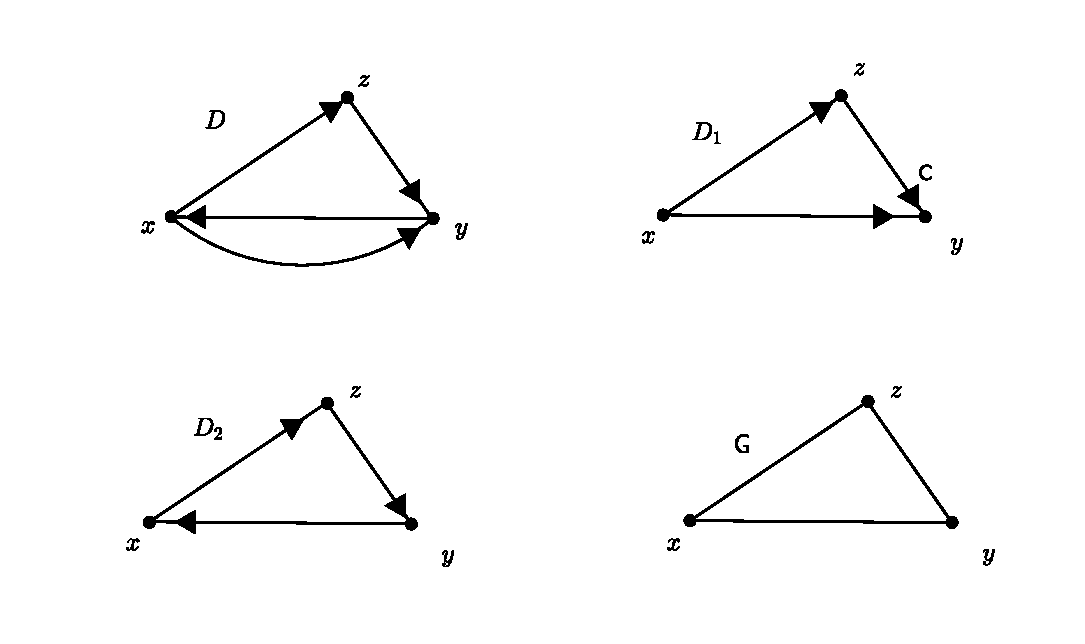
\includegraphics[scale=0.55]{digraphs.eps}
\caption{$D$ is a generic digraph;
		$D_1$ is an acyclic oriented graph;
		$D_2$ is a directed cycle;
		$G$ is the underlying graph of $D,D_1,D_2$}\label{digraph}
\end{figure}


A sequence $x_0,...,x_n$ of distinct vertices of a digraph $D$ is a \textit{(directed) path} if for any $i$ $(x_i,x_{i+1})$ is an arc of $D$; a path in which $x_n$ coincides with $x_0$ is called \textit{directed cycle}. Note that Fig. \ref{digraph} shows that an acyclic oriented graph may have an underlying graph with a cycle. As simple graphs have spanning trees and they are easy to obtain, digraphs have spanning acyclic digraphs; they also have a maximality property, i.e. whichever arc is added, it creates a directed cycle.

\newpage
\begin{lemma}[\textbf{Spanning acyclic digraph}]
Let $D=(V,A)$ be a connected digraph; then there is an acyclic oriented cycle $T$ which is connected and obtained by $D$ only by removing arcs.
\end{lemma}

The orientations of a simple graph can be useful to find the chromatic number. A characterization of $\chi (G)$ was found independently by L.M. Vitaver \cite{vitaver}(1962), M. Hasse \cite{hasse}(1963), B. Roy \cite{roy}(1967), T. Gallai \cite{gallai}(1969); here I will show the proof given by Chartrand and Zhang in their book \cite{chrom}, and later I will show the method adopted by Matijasevi\v{c} \cite{mat-1} which uses hyper-resolution.
\begin{definition}\label{prova}
Let $G$ be a simple graph and $D$ an orientation of $G$;\\ we define $\ell (D)$ as the length of a longest directed path of $D$
\end{definition}
\begin{proposition}\label{prop-vitaver-easy}
There is an orientation $D$ of $G=(V,E)$ such that $$ \chi (G) \geq 1+\ell(D) $$
\end{proposition}

\textit{Proof:}  We take a coloring map $c:V\rightarrow \{1,...,\chi (G)\}$, we build an orientation
 $D$ choosing a direction for each edge $uv$ of $G$, in particular we pick the arc 
 $(u,v)$ if $c(u)< c(v)$. In such orientation, any path is long at most $\chi 
 (G)-1$ whence $\ell(D)\leq \chi (G)-1  $, that is $ \chi (G) \geq 1+\ell(D) $ 
\QED

\begin{theorem}[The Gallai-Hasse-Roy-Vitaver theorem]\label{vitaver}
For every orientation $D$ of a graph $G=(V,E)$ $$\chi (G)\leq 1 + \ell(D)$$
\end{theorem}
\textit{Proof: }Let $D$ be an orientation of $G$ and $D'$ a spanning acyclic subdigraph of $D$, we define a coloring map $c$ on $G$ by assigning to each vertex $v$ the color 1 plus the length of the longest directed path of $D'$ that ends in $v$. Clearly the number of colors used is $1+\ell(D)$, indeed the longest path of $D'$ is also in $D$, otherwise $D'$ would not be maximal. 

Thus it remains to show that $c$ is a proper coloring, i.e. that if $uv\in E$, $c(u)\neq c(v) $, to this aim consider an arc $(u,v)$ of $D$, if it is also an arc of $D'$ then $c(u)<c(v)$; otherwise if it is not in $D'$, adding it creates a directed cycle which is the case only if there is a path from $v$ to $u$, thus $c(v)<c(u)$ \QED

\noindent The following result characterizes the chromatic number of simple graphs and is a direct consequence of the last propositions.
\begin{corollary}\label{cor-vitaver}
Let $G$ be a graph and $\ell$ the minimum possible value of $\ell(D)$, $D$ orientation of $G$; then   
$$\chi (G)=1+\ell$$
\end{corollary}

\textit{Proof:}
Let $D$ be an orientation of $G$ such that 
$$\ell(D)=\ell=\textrm{min}\{\ell(D') \; 	,D' \textrm{ orientation of } G\}$$ 
then by Theorem \ref{vitaver} $\chi(G) \leq 1+\ell$. On the other hand by Proposition \ref{prop-vitaver-easy} for some orientatin $D'$  of $G$, $\chi(G)\geq 1+\ell(D')$; therefore, since $\ell(D')\geq\ell$ 
$$\chi (G)=1+\ell$$\QED

 
The figure \ref{fig-vitaver} displays how the Gallai-Hasse-Roy-Vitaver theorem applies to a cycle of length five, there are shown four different orientations of the cycle and to each vertex is assigned a color based on how long is the longest directed path that reaches it. The rightmost orientation is not acyclic, every vertex is reached by a directed path of length five and they would all receive the same color. The leftmost orientation is one that achieves the minimum $\ell(D)$, which in the case of odd cycles is 2, and the chromatic number of odd cycles is 3
\vspace{2cm}
\begin{figure}[h]
\centering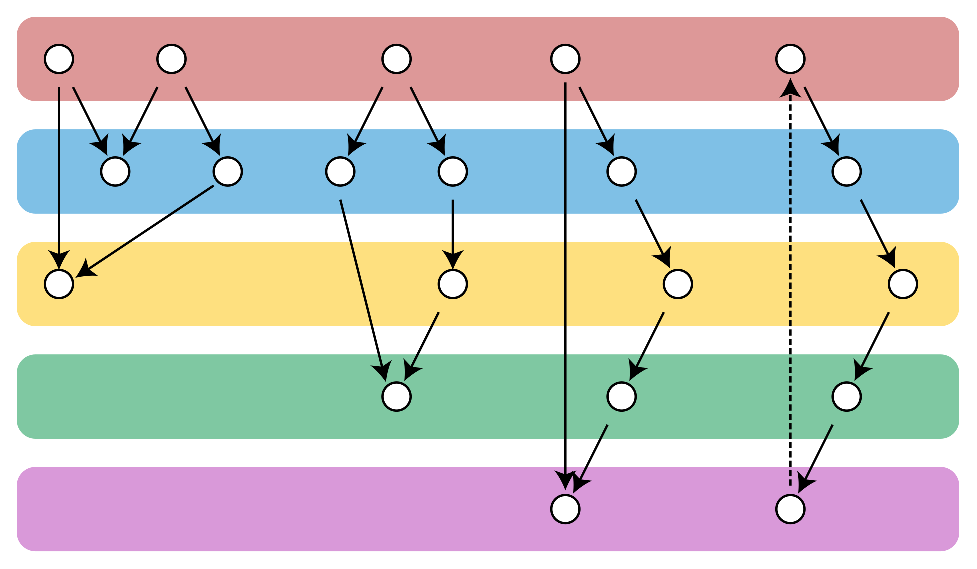
\includegraphics[scale=0.7]{vitaver.eps}
\caption{ }\label{fig-vitaver}
\end{figure}

\newpage
\section{Hyper-resolution approach to coloring}
Every coloring can be uniquely described (up to renaming the colors) by the symmetric binary relation "vertices $x$ and $y$ have the same color", which we denote by  $\E xy$. 
Such binary relation, in order to represent a coloring map, should respect a symmetry axiom, a transitivity axiom, and be false whenever the two vertices are adjacent 
\begin{gather}
\E xy \rightarrow \E yx \label{symmetry-axiom}\\
\E xy \wedge \E yz \rightarrow  \E xz \label{color-prop1}\\
( xy \in E \Rightarrow ) \qquad  \neg \E xy \label{color-prop2}
\end{gather}
Also for an $n$-coloring we require that whenever we pick $n+1$ vertices, at least 2 of them must share the color, which amounts to require for any $\{ x_0, x_1, ... , x_n \} \subseteq  V$
\begin{equation} \label{color-prop3}
\bigvee_{i=0}^{n-1} \bigvee_{j=i+1}^{n} \E x_i x_j
\end{equation}
Conversely if a binary symbol satisfies the above axioms, then it corresponds to some coloring map. More formally, for every graph $G=(V,E)$, we consider the language $\mathscr{L}=\{\E\}\cup V\cup E$, where $\E$ is a binary relation symbol, and $V\cup E$ contains the constants. The models of the formulae (\ref{symmetry-axiom})-(\ref{color-prop3}) are the $n$-colorable graphs that contain $G$; and if $G$ is not $n$-colorable, then  the axioms are inconsistent and there are no models. 
\begin{definition}
Let $G$ be a simple graph and $n$ a positive natural number; then we call $C_{G,n}$ the set of all possible formualae of the form (\ref{color-prop1}), (\ref{symmetry-axiom}), (\ref{color-prop2}), and (\ref{color-prop3}). The resolution calculus that comes from $C_{G,n}$ is denoted as $H_{G,n}$.
\end{definition}
The hyper-resolution calculus $H_{G,n}$ has the following rules
\begin{equation}
\label{symm}
\prftree{\Gamma \cup \E xy }{ \Gamma\cup \E yx }
\end{equation}
\begin{equation}
\label{trans}
 \prftree{\Gamma \cup \E xy }{\Delta \cup \E yz }{\Gamma \cup \Delta \cup \E xz }
\end{equation}
\begin{equation}
\label{jred}
\prftree[r]{$\quad xy \in E $}{\Gamma \cup \E xy }{ \Gamma}
\end{equation}
\begin{equation}
 \label{ax-col}
\prftree{\Gamma}{ \Gamma \cup \{\E x_0 x_1 , ... , \E x_{n-1} x_n  \}}
\end{equation}
Note that, since (\ref{ax-col}) is the only rule with empty premise, any tree made in $H_{G,n}$  has (\ref{ax-col}) as leaves. The following lemma ensures that every tree can be rearranged in such a way that the rules appear in a precise order: First the literals are introduced from $\emptyset$ by the rule (\ref{ax-col}); second all the symmetry rules (\ref{symm}) apply, followed by the transitivity rule (\ref{trans}); last literals are eventually removed by the elimination rule (\ref{jred}).


\begin{lemma}\label{lemma_rules}
For any derivation in $H_{G,n}$, there is a tree that respects the following
\begin{itemize}
\item[1)] (\ref{ax-col}) is preceded only by other applications of (\ref{ax-col}); also if the derivation has no trivial application, then (\ref{ax-col}) appears only at leaves.
\item[2)] (\ref{symm}) is preceded only by applications of (\ref{symm}) or (\ref{ax-col})
\item[3)] (\ref{trans}) is not preceded by  applications of (\ref{jred})
\item[4)] (\ref{jred}) is followed only by  applications of (\ref{jred})
\end{itemize}\end{lemma}
\noindent\emph{Proof:}

\noindent 1) Suppose to have a rule $x$ that precedes (\ref{ax-col}), switch them in the following way. 

%% axiom colors and any rule
\begin{eqnarray*}
\prfrulenameskip=0.4em\prflinepadbefore=1ex
\prftree[r]{(\ref{ax-col})}{
\prftree[r]{$x$}{\Gamma}{\qquad\Delta}{\qquad\Sigma\qquad}
}{\Sigma\cup\{\E x_0 x_1 , ... , \E x_{n-1} x_n  \}}
& \leadsto
&\prftree[r]{$x$}{
\prftree[r]{(\ref{ax-col})}{\Gamma}{\Gamma\cup\{\E x_0 x_1 , ... , \E x_{n-1} x_n  \}}
}{\qquad\Delta\qquad\quad}{\Sigma\cup\{\E x_0 x_1 , ... , \E x_{n-1} x_n  \}}
 \end{eqnarray*}
Here $\Delta$ is the second premise in the case that $x$ is (\ref{trans}), otherwise it should be dropped. Also, if the tree has  no trivial application, (\ref{ax-col}) cannot be preceded by anything and it must be a leaf. Indeed, if we apply (\ref{ax-col}) to a non empty clause $\Gamma$, such application is trivial since $\emptyset\in\Gamma$.
 
\noindent 2) Because of point 1, we can always achieve a tree where (\ref{ax-col}) is never applied below (\ref{symm}), it remains to check the case when  (\ref{trans}) or (\ref{jred}) precedes (\ref{symm}).

% symmetria e trans
\begin{eqnarray*}
\prfrulenameskip=0.4em\prflinepadbefore=1ex
\prftree[r]{(\ref{symm})} {\prftree[r]{(\ref{trans})}{\Gamma\cup \E ab  }{\Delta\cup \E bc}
{\Gamma\cup\Delta\cup \E ac } 
 }{\Gamma\cup\Delta\cup\E ca } 
& \leadsto
&\prftree[r]{(\ref{trans})} 
 { \prftree[r]{(\ref{symm})}{\Delta\cup\E bc } { \Delta\cup\E cb  } }
 {\prftree[r]{(\ref{symm})}{\Gamma\cup\E ab} { \Gamma\cup\E ba  } }
{\Delta\cup\Gamma\cup\E ca}
 \end{eqnarray*}


%eliminazione e simmetria 
\begin{eqnarray*}
\prfrulenameskip=0.4em\prflinepadbefore=1ex
\prftree[r]{(\ref{symm})} 
{\prftree[l,r]{(\ref{jred})}{$xy \in E$}{\Gamma \cup \{\E xy ,\E ab \}}{\Gamma \cup \E ab }}
{\Gamma  \cup \E ba }
& \leadsto
&\prftree[l,r]{(\ref{jred})}{$xy \in E$} 
{\prftree[r]{(\ref{symm})}
{\Gamma \cup \{\E xy ,\E ab \}}
{\Gamma\cup \{\E xy , \E ba \} }}
{\Gamma \cup \E ba }
 \end{eqnarray*}



\noindent 3) From point 1 and 2, we know that there is a tree in which the transitivity rule (\ref{trans}) cannot be followed by (\ref{ax-col}) nor (\ref{symm}). It remains to show how to rearrange it when (\ref{jred}) precedes (\ref{trans})

% eliminazione e trans
\begin{eqnarray*}
\prfrulenameskip=0.4em\prflinepadbefore=1ex
\prftree[r]{(\ref{trans})} 
{\prftree[l,r]{(\ref{jred})}{$xy \in E$}{\Gamma \cup \{\E xy ,\E ab \}}{\Gamma \cup \E ab }}
{ \prfassumption{\Delta \cup \E bc  }}
{\Gamma \cup \Delta \cup \E ac }
& \leadsto
&\prftree[l,r]{(\ref{jred})}{$xy \in E$} 
{\prftree[r]{(\ref{trans})}
{\Gamma \cup \{\E xy ,\E ab \}}{\Delta \cup \E bc }
{\Gamma\cup\Delta \cup \{\E xy , \E ac \} }}
{\Gamma \cup \Delta \cup \E ac }
 \end{eqnarray*}

\noindent 4) If a derivation respects all the previous points, then the elimination rule (\ref{jred}) is either the last one or is followed only by other applications of itself. Indeed if another rule follows the elimination one, either the point 1, 2 or 3 does not hold.

\QED


\subsection*{Bipartite graphs}
\addcontentsline{toc}{subsection}{Bipartite graphs}
Now we see, using resolution methods, that a graph is bipartite  if and only if it does not contain odd cycles. First we show that any graph $G$ with an odd cycle is not 2-colorable and therefore not bipartite; this can be done by directly showing that the empty set can be derived in $H_{G,2}$. 
Second, that whenever a graph $G$ is not 2-colorable, there is an odd cylce in $G$. This second proof relies on Robinson's Theorem and is constructive; given a non bipartite graph, it shows how to build an odd cycle which is a subgraph of it. 

\begin{proposition}
Let $G=(V,E)$ be a graph that contains an odd cycle; then $G$ is not 2-colorable 
\end{proposition}
\textit{Proof:}
We show that if there is an odd cycle in $G$, then the empty clause is derivable in $H_ {G,2}$, i.e. $\vdash_{H_{G,2}} \emptyset$, and that therefore the axioms \ref{symmetry-axiom} ,\ref{color-prop1}, \ref{color-prop2} and \ref{color-prop3} are inconsistent.

Let $x_1, ..., x_{2n+1} $ be an odd cycle, by definition for $i=1,2,..., 2n$ $x_i x_{i+1} \in E$ and $ x_{2n+1} x_1 \in E$. For $i=1,2,...,2n-1$ consider the tree $\D_i$ in $H_{G,2}$:

$$
\prftree[r,l]{(\ref{jred})}{$x_{i+1} x_{i+2} \in E$}{
\prftree[r,l]{(\ref{jred})}{$x_i x_{i+1} \in E$} 
{ \prftree[r]{(\ref{ax-col})}{\emptyset}
{\{\E x_i x_{i+1} , \E x_{i} x_{i+2} , \E x_{i+1} x_{i+2}\}}}
{\{ \E x_{i} x_{i+2} , \E x_{i+1} x_{i+2}  \}}
}
{\E x_i x_{i+2}}
$$
\newpage Using the trees $\D_1,...,\D_{2n-1}$, we obtain the following derivation of the empty set in $H_{G,2}$:
$$
\prftree[r,l]{(\ref{jred})}{$x_{2n+1}x_1\in E$}
{ \prftree[r]{(\ref{symm})}
{\prftree[r]{(\ref{trans})} 
{\prftree{ \prftree[l]{(\ref{trans})}{ \prfsummary{\D_1} {\E x_1x_3}  }{  \prfsummary{\D_3}{\E x_3x_5} }
{\E x_1 x_5}}{\prfsummary{ \D_5}{ }}{ \prfsummary{...}{} }{\prfsummary{ \D_{2n-3}}{ }}
{ \E x_1 x_{2n-1}}}{\prfsummary{\D_{2n-1}} { \E x_{2n-1}x_{2n+1}}}
{\E x_1 x_{2n+1} } }  
{\E x_{2n+1}x_1} }
{\emptyset}
$$
\QED

The idea shown by the last tree is that, if the graph is 2-colorable with a ($2n+1$)-cycle and $c$ is a 2-coloring map, whenever we pick three consecutive vertices $x_i,x_{i+1},x_{i+2}$ of the cycle, two of them must be of the same color and since adjacent vertices have different colors, we have $c(x_i)=c(x_{i+2})$; whence $c(x_1)=c(x_3)=c(x_5)=...=c(x_{2n+1})$ which is impossible since $x_{2n+1}x_1 \in E$.

The opposite direction is less trivial, and the proof requires  Robinson's theorem; before showing it, we need the following lemma about odd cycles.

\begin{lemma}\label{tech-lemma-graph}
Let $C_1=(V_1,E_1)$ and $C_1=(V_2,E_2)$ be two odd cycle such that $xy\in E_1\setminus E_2$ and 
$yz\in E_2\setminus E_1$;  then the graph $G=(V_1\cup V_2, E_1\cup E_2\setminus\{xy,yz\}\cup\{xz\})$ contains an odd cycle.
\end{lemma}
\textit{Proof:} 
Let $2n+1$ and $2m+1$ respectively the length of $C_1$ and $C_2$, if $y$ is the only vertex in the intersection,	 by removing the edges $xy,yz$ and adding $xz$ we get a cycle in $G$ of length $2(n+m)+1$. 
\begin{figure*}[h]
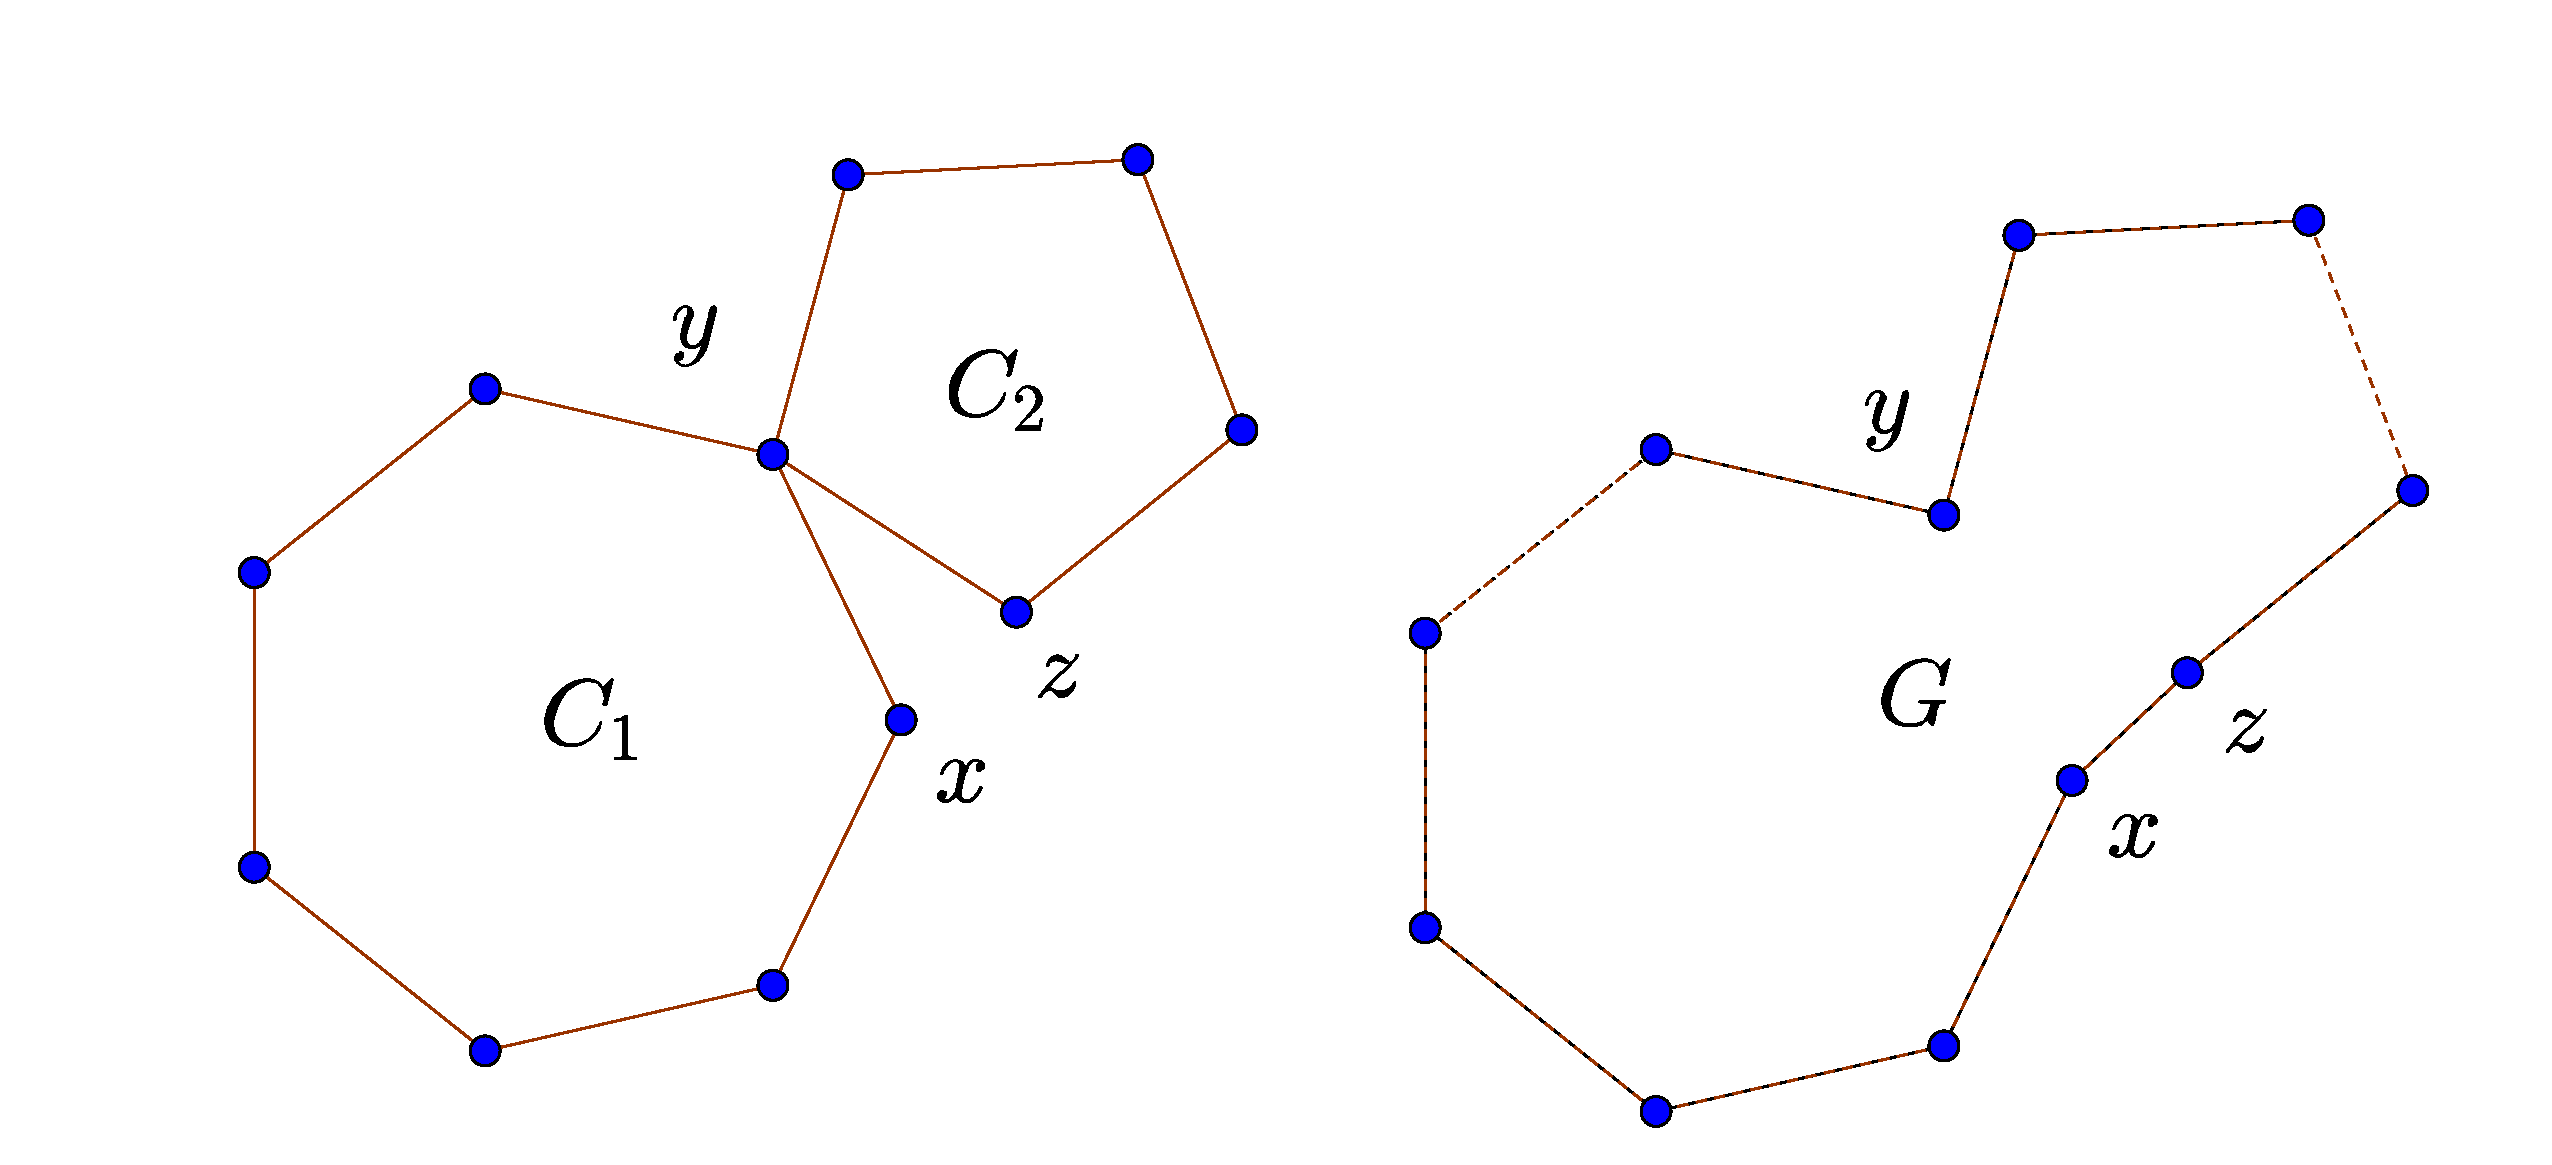
\includegraphics[scale=0.23]{oddcycles1.eps}
\end{figure*}

\newpage
It remains to consider when $C_1$ and $C_2$ intersect multiple times, let $P$ and $Q$ be the longest path respectively of $C_1$ and $C_2$ with $y\in P\cap Q$ and where the only vertices that belong to $V_1\cap V_2$ are the endpoints of the paths.
Then $P\cup Q$ is a cycle that passes trough the edges $xy$ and $yz$, if the length of such cycle is even, by removing $xy,yz$ and adding $xz$ we get an odd cycle in $G$.

\begin{figure}[h]
\centering
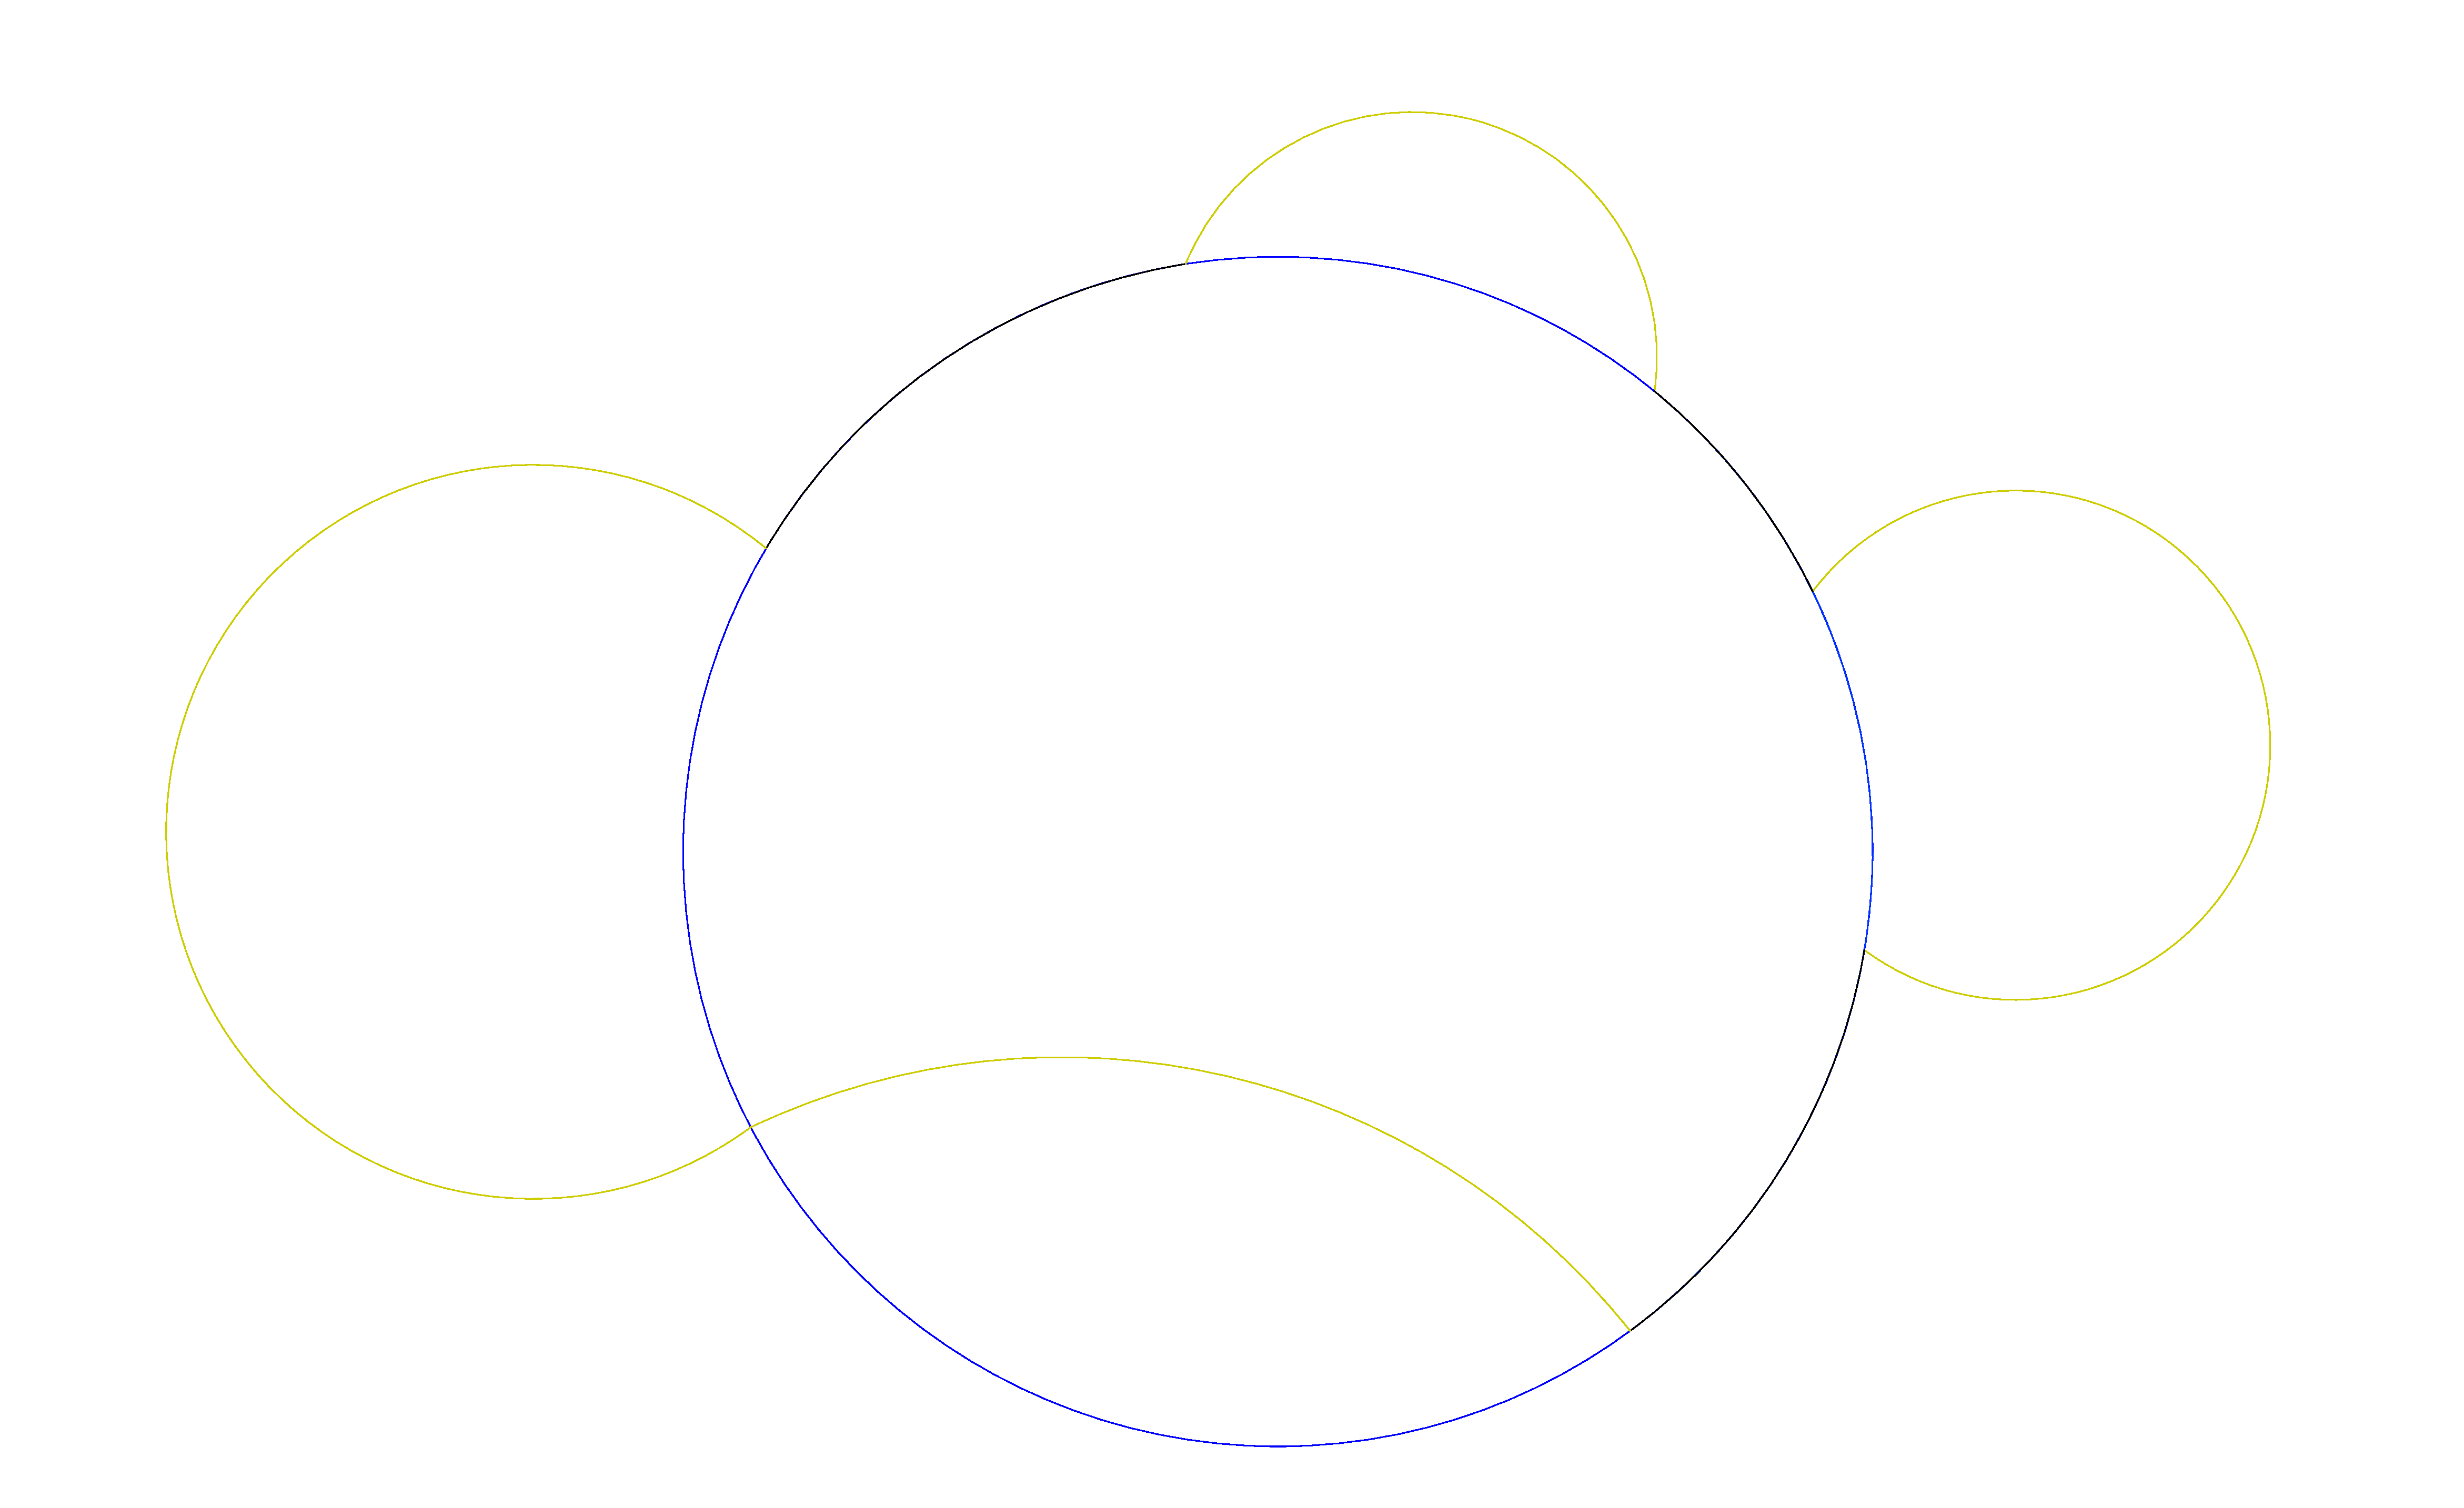
\includegraphics[scale=0.5]{oddcycles-interceptions.eps}
\caption{In blue $C_1 \backslash C_2 $, in green $C_2\backslash C_1 $ and in black the intersection }
\end{figure}
If $P\cup Q$ is an odd cycle, consider the remaining part which namely consists of $C_1\cap C_2$ and of $\tilde{C}_1,..,\tilde{C}_l$ cycles, then at at least one of them must be odd since $|P\cup Q|$ is odd and the following holds $$2n+1+2m+1-|P\cup Q| = \sum^l_{i=1} length(\tilde{C}_i) + 2\cdot |V_1\cap V_2|   $$
Finally, since $xy\in P$ and $yz\in Q$, such odd cycle is also in $G$. 
\QED



\begin{proposition} \label{mio}
If a graph $G=(V,E)$ is not 2-colorable, then it has an odd cycle
\end{proposition}
\textit{Proof:}
If $G$ is not 2-colorbale, also every graph that contains $G$ is not 2-colorable; therefore by Robinson's Theorem, we know that  $\vdash_{H_{G,2}} \emptyset$. Consider a derivation of $\emptyset$  that respects Lemma \ref{lemma_rules}, in particular that it does not have trivial application, and all the applications of the elimination rule (\ref{jred}) are close to the root.
Now we proceed by induction on the number $k$ of applications of the transitivity rule (\ref{trans}).
If $k=0$ the tree is of the form:
\begin{eqnarray*}
\prftree[r,l]{(\ref{jred})}{$xy \in E$}{
\prftree[r,l]{(\ref{jred})}{$yz \in E$}{
\prftree[r,l]{(\ref{jred})}{$xz \in E$}{
\prftree[r]{(\ref{ax-col})} { }{ \{ \E xy , \E yz, \E xz  \} } } 
{\{ \E xy , \E yz \} } } 
{ \E xy  } }
{ \emptyset }
\end{eqnarray*}
Then $xy,xz,yz \in E$ and the 3-cycle $xyz$ is a subgraph of $G$.
 
For $k >0$ the tree is of the following form, 
$$
\prftree[r]{(\ref{trans})}
{\prfsummary[$\D_1$]{\emptyset}{\Gamma_1 \cup \E xy }}
{\prfsummary[$\D_2$]{\emptyset}{\Gamma_2 \cup \E yz }}
{\prfsummary{\Sigma \cup \E xz }{\emptyset}}
$$
Every literal in $\Sigma\cup\E xz$ is eliminated by rule (\ref{jred}), which means that the corresponding edge is in $E$. Since there are no trivial applications, $\E xy \notin \Gamma_1 $ and $\E yz \notin \Gamma_2 $, and for any $\E ab \in \Gamma_i$, $ab \in E$, whence we have the derivations $\D'_i:\,\Gamma_i \vdash_{H_{G,2}} \emptyset$. 
\newpage
Let $E'=E\cup\{xy,yz\}$ and $G'=(V,E' )$ ; then the derivations $\D_i$ and $\D'_i$ are valid also in $H_{G',2}$. Thus we have the two following trees in  $H_{G',2}$ :
\begin{eqnarray*}
\prfsummary[$\D'_1$]{
\prftree[r]{$xy \in E'$}{\prfsummary[$\D_1$]{\emptyset}{\Gamma_1 \cup \E xy}}{\Gamma_1}}
{\emptyset}
&\prfsummary[$\D'_2$]{
\prftree[r]{$yz \in E'$}{\prfsummary[$\D_2$]{\emptyset}{\Gamma_2 \cup\E yz}}{\Gamma_2}}
{\emptyset}
\end{eqnarray*}
In both trees the number of applications of the rule (\ref{trans}) is certainly less than $k$; then by induction hypothesis $G'$ has two odd cycles $C_1$ and $C_2$. If $C_1=C_2$, $\E xy \in \Gamma_2$, and $\E yz \in \Gamma_1$, whence $xy,yz\in E$ and $C_1$ is also in $G$.
\\Let $E_i$ be the set that contains the edges of $C_i$, such sets cannot coincides otherwise $C_1=C_2$.
If $xy,yz \notin E_1$, then $E_1\subseteq E$ and $C_1$ is a cycle of $G$. 

Thus suppose is not the case that $xy,yz \notin E_1$, i.e. $xy \in E_1 \o yz\in E_1 $. Suppose first that $yz\in E_1$, then $\E yz\in\Gamma_1$ and $yz\in E$; if $xy\notin E_2$, then $E_2\subseteq E$, otherwise $\E xy \in \Gamma_2$ and $xy\in E$, in both cases  $E_2\subseteq E$ and $G$ contains $C_2$. Therefore it remain 
the case $yz\notin E_1 \e xy\in E_1$. Similarly we can conclude  $yz\in E_2 \e xy\notin E_2$, whence $xy\in E_1\setminus E_2$ and $yz\in E_2\setminus E_1$

Finally we can apply Lemma  \ref{tech-lemma-graph}, the resulting graph is a subgraph of $G$ since $E_1\cup E_2\setminus\{xy,yz\}\cup\{xz\} \subseteq E $, and therefore it has the required odd cycle. 
\QEDn

\newpage
\subsection*{Gallai-Hasse-Roy-Vitaver theorem}
\addcontentsline{toc}{subsection}{Gallai-Hasse-Roy-Vitaver theorem}

Another way to describe a proper coloring of a graph, is by introducing a partial order on the colors, indeed we may use the binary symbol $<$ and write $x<y$ to say "the vertex $x$ is colored in a color smaller than the one of the vertex $y$". We shall write $x\geq y $ instead of $\neg (x<y)$. The role of the formulas (\ref{color-prop1}), (\ref{color-prop2}) and (\ref{color-prop3}) is now played by 

\begin{gather}
x\geq x\\
x<y \e y<z \rightarrow x<z \\
( xy \in E \Rightarrow ) \qquad  x<y \o y<x\\
\bigvee_{i=0}^{n-1} x_i\geq x_{i+1}
\end{gather}
In the formalism of hyper-resolution, for a given graph $G=(V,E)$ we consider the language $\mathscr{L}=\{\geq\}\cup V\cup E$, where $V\cup E$ are constants; the models are the $n$-colorable graphs that contain $G$ while the inference rules are
\begin{align*}
\prftree{\Gamma}{\Gamma \cup x\geq x }\qquad \qquad\qquad
& \qquad\prftree{\Gamma\cup x\geq y}{ \Sigma\cup y\geq z }{\Gamma\cup\Sigma\cup x\geq z } \\
\,&\,\\
\prftree[l]{$\quad xy \in E $}{\Gamma \cup  x\geq y }{\Sigma \cup  y\geq x }
{ \Gamma\cup\Sigma} \qquad &\qquad \prftree{\Gamma}
{\Gamma\cup\{x_0\geq x_1 ,..., x_{n-1}\geq x_n \}}
\end{align*}
The advantage of these rules with respect to the previous approach can be seen in the last rule, indeed now to describe a $n$-coloring it's enough to have an axiom that introduces $n-1$ literals while with (\ref{color-prop3}) we must involve $n(n+1)/2$ vertices for each instance.


Now, fix a simple graph $G$ and an orientation $D$ of $G$, we want to describe the property of Vitaver's theorem "The directed paths in $D$ are not longer than $\ell (D)$" where $\ell (D)$ is defined to be the length of the longest directed path in $D$, maintaining the same notation as in Theorem \ref{vitaver}. To formalize such property we introduce the binary relation symbol \pred which is defined on pairs of vertices and which indicates the existence of a directed path from one vertex to the other
$$ x\pred y \Leftrightarrow \textrm{There is a path from } x\textrm{ to } y $$
Since every arc can be seen as a path of length one, if there is an edge $xy$ in the underlying graph $G=(V,E)$ of $D$, then it's necessary  to have
\begin{equation}\label{pred1}
xy\in E \Rightarrow  x\pred y \o y\pred x
\end{equation}
If the end of the path is the start of another path, there exists a path which is the concatenation of the two:
\begin{equation}\label{pred2}
x\pred y \e y\pred z \rightarrow x\pred z
\end{equation}
Also, requiring that $\ell (D)$ is the maximum length of a path is equivalent to ask that there are no paths of length equal to $n=\ell (D)+1$, which amounts to ask for any set of $n+1$ vertices
$$ \neg(x_0\pred x_1 \e x_1 \pred x_2 \e ...\e x_{n-1}\pred x_n )$$
and if we denote $\neg (x\pred y)$ as $x \npred y$ 
\begin{equation}\label{pred3}
x_0\npred x_1 \o x_1\npred x_2 \o ...\o x_{n-1}\npred x_n
\end{equation}
Finally, we require $D$ to be an acyclic orientations of $G$, which amounts to say that for any vertex $x$ there is no path from $x$ to $x$, that is:
\begin{equation}\label{pred4}
x\npred x
\end{equation}

Thus if we consider the language  $\mathscr{L}=\{\npred\}\cup V\cup E$, the models are the acyclic orientation of a subgraph of $G$ and the rules of inference are
\begin{align*}
\prftree{\Gamma}{\Gamma \cup x\npred x }\qquad \qquad\qquad
& \qquad\prftree{\Gamma\cup x\npred y }{ \Sigma\cup y\npred z  }{\Gamma\cup\Sigma\cup x\npred z } \\
\,&\,\\
\prftree[l]{$\quad xy \in E $}{\Gamma \cup  x\npred y }{\Sigma \cup  y\npred x }
{ \Gamma\cup\Sigma} \qquad &\qquad \prftree{\Gamma}
{\Gamma\cup\{x_0\npred x_1 ,..., x_{n-1}\npred x_n \}}
\end{align*}
Clearly the rules have the same shape as the ones given for $\geq$. We can therefore conclude that $\npred$ describes an $n$-coloring for $G$ where
$$n=1+\min\{\ell(D'), D' \textrm{ spanning acyclic digraph of an orientation } \textrm{ of }G\}$$
If we consider an orientation $D$ of $G$ and a spanning acyclic digraph $D'$ of $D$, we have $\ell (D') \leq \ell(D)$ whence $n\leq 1+ \ell $ where $\ell$ is  $\min\{\ell(D), D \textrm{ orientation of }G\}$ as in corollary \ref{cor-vitaver}.
Finally recalling that Proposition \ref{prop-vitaver-easy} says that for some orientation $D$
$$\chi (G) \geq 1+ \ell (D)$$
we reach the same conclusion of Corollary \ref{cor-vitaver}, i.e. 
$$\chi (G) = 1+\ell$$

\newpage
\subsection*{$\mu_n$ graphs}
\addcontentsline{toc}{subsection}{$\mu_n$ graphs}
The $\mu_n$ graphs are a family of graphs defined by Matiyasevich \cite{mat-2} with the purpose to characterize the graphs that cannot be colored in $n$ colors. 
Such graphs are built starting from the complete graphs with $n+1$ vertices, which is not $n$ colorable; 
and every step of the construction ensures that the result is still not $n$ colorable. Matiyasevich's theorem tells us that every graph that cannot be colored in $n$ colors, contains a $\mu_n$ graph.
They are defined by induction as follows

\begin{definition}\label{def_mun}
$\mu_n-graph$
\end{definition}
\begin{itemize}
\item[-] Every complete graph with $n+1$ vertices is a $\mu_n$-graph
\item[-] If $G_1=(V_1,E_1)$ and $G_2=(V_2,E_2)$ are $\mu_n$-graphs and $a,b,c$ are distinct vertices such that
$$ a,b\in V_1 \quad b,c\in V_2  $$
$$ ab\in E_1, ab\notin E_2 \qquad  bc\in E_2, bc\notin E_1$$
Then the graph $G=(V_1\cup V_2, E_1\cup E_2\cup\{ac\} \setminus\{ab,bc\} )$ is a $\mu_n$-graph.
\end{itemize} 

To the best of our knowledge, in the literature there are no other graphs defined in such a way; although we have found the $\mu_n$ graphs can be constructed using splitting methods which were introduced by Fleischner (1990) \cite{split}.

The $\mu_1$ graphs are of little interest. The complete graph with two vertices, $K^2$, is a single edge; when two edges are composed according to the definition, the result is a single edge. Thus all $	\mu_1$ graphs are single edges; and every graph that contains  an edge, contains a $\mu_1$ graph. Clearly $\mu_1$ graphs are not 1-colorable; and graphs that are not 1-colorable contain at least one edge.

$\mu_2$ graphs are more interesting; they characterize bipartite graphs, and can give a better insight of generic $\mu_n$ graphs. Clearly all the odd cylces are $\mu_2$ graphs; on the other hand, not all $\mu_2$ graphs are odd cycles, the following example shows a $\mu_2$ graph which is not a cycle and which can be built using the definition and starting by a 3-cycle and a 5-cycle 
\begin{figure*}[h]
\centering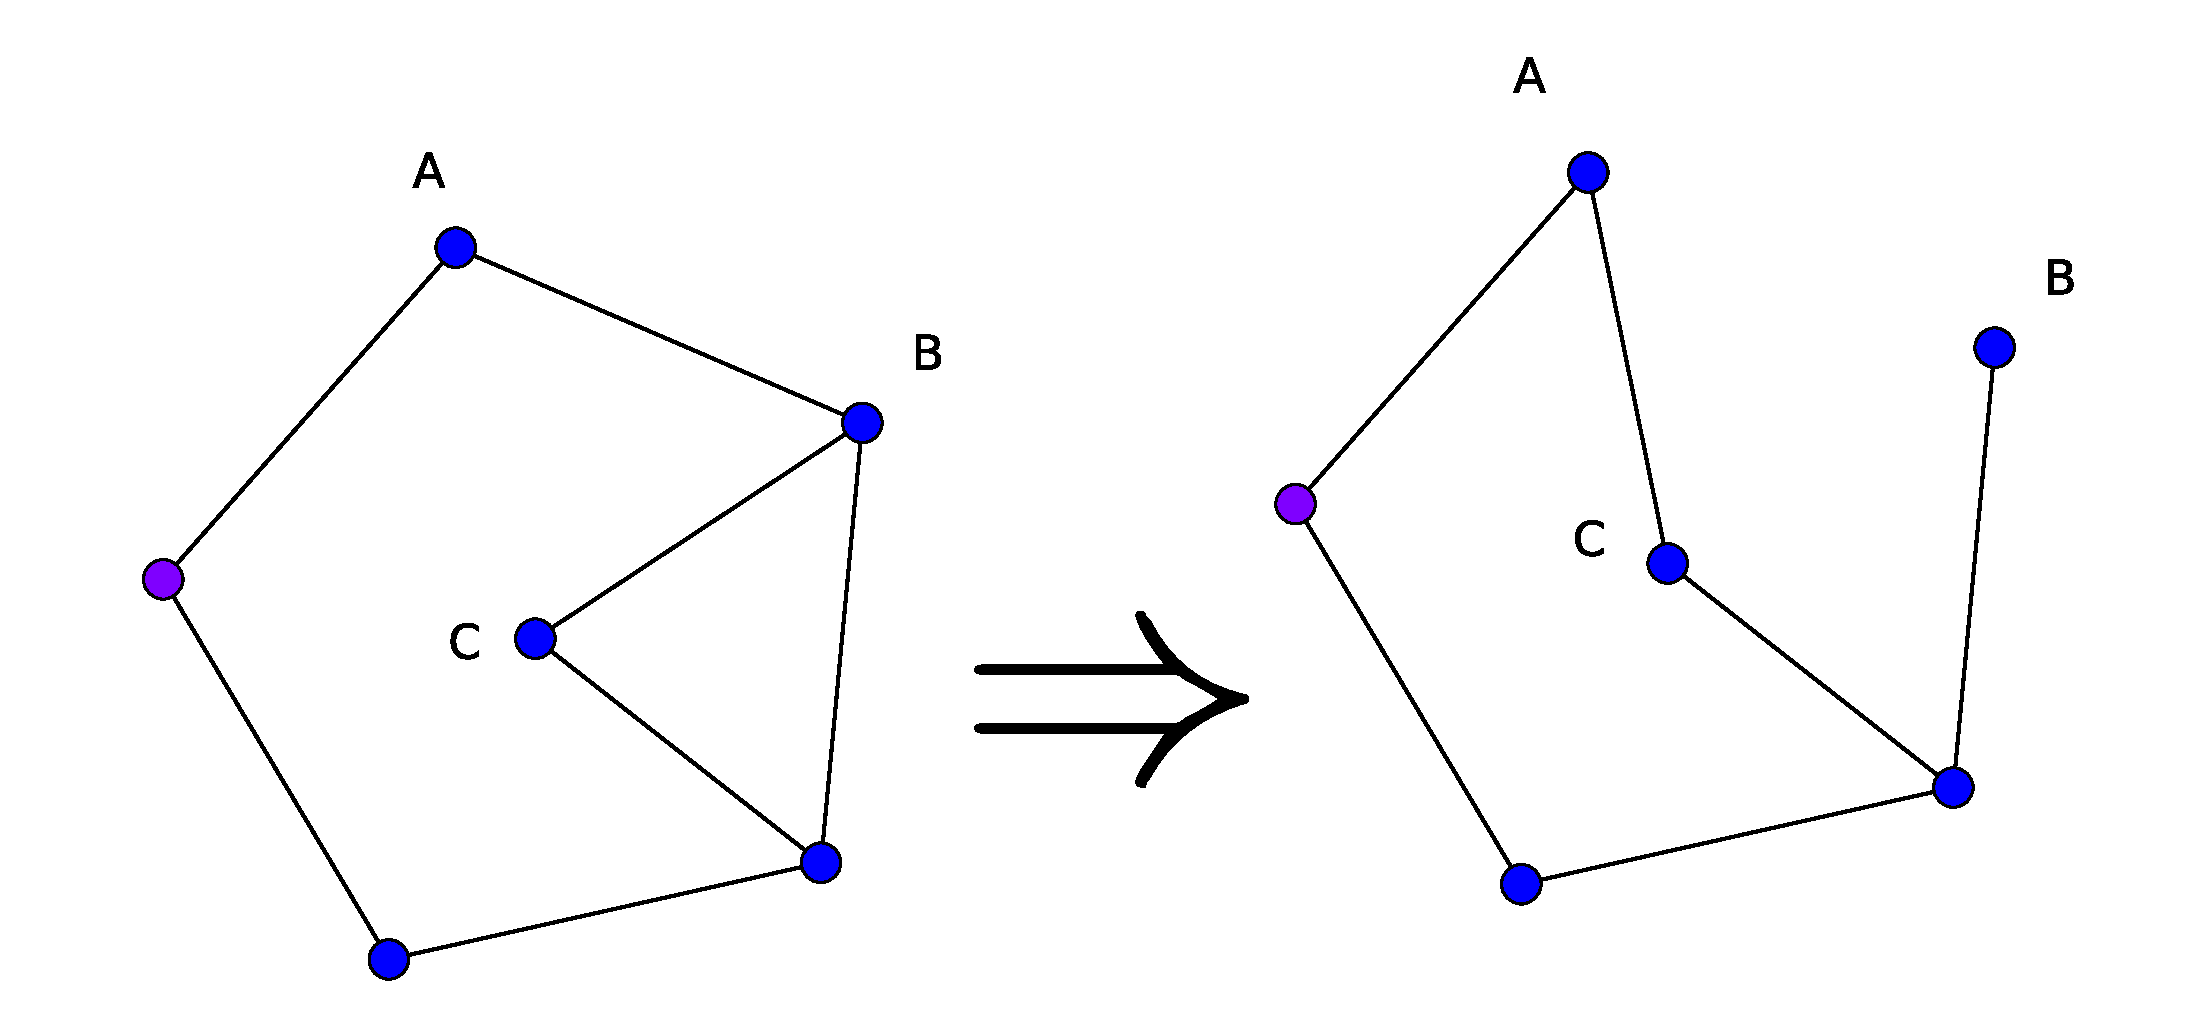
\includegraphics[scale=0.25]{mu2.eps}
\end{figure*}

\noindent They do not even need to be connected, indeed starting from two $\mu_2$ graphs of the kind shown above, we obtain a $\mu_2$ graph with an isolated vertex.

\begin{figure*}[h]
\centering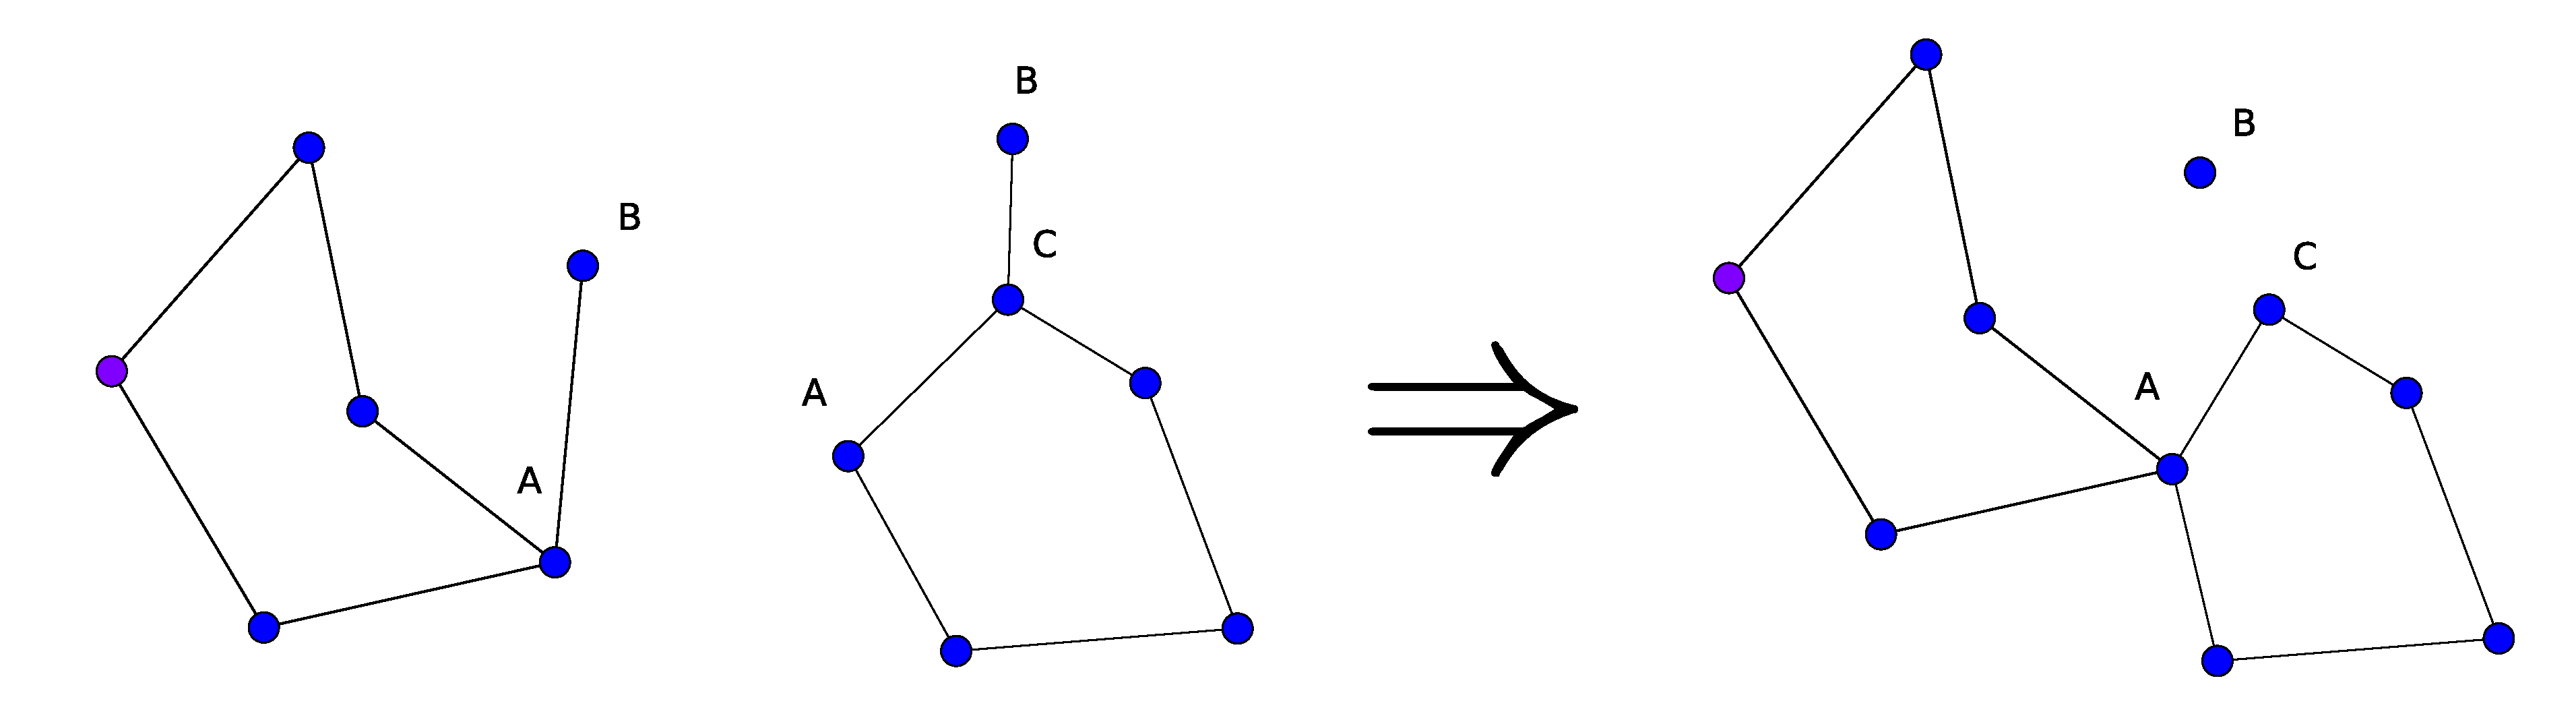
\includegraphics[scale=0.25]{mu2-con1.eps}
\end{figure*}

\noindent The examples suggest that $\mu_2$ graphs always contain an odd cycle, this can be readily proved thanks to Lemma  \ref{tech-lemma-graph}, which was used to prove that  non bipartite graphs have at least an odd cycle.
\begin{proposition}\label{contains-odd}
Let $G$ be $\mu_2$ graph; then it contains an odd cycle.
\end{proposition}

\textit{Proof:} 
We proceed by induction on the number of vertices $n$. If $n=3$, the only $\mu_2$ graph is the complete graph which is a 3-cycle. If $n>3$, let $G_1=(V_1,E_1)$, $G_2=(V_2,E_2)$, and $G=(V_1\cup V_2, E_1\cup E_2\cup\{ac\} \setminus\{ab,bc\} )$ as in Definition \ref{def_mun}. 
\\By induction hypothesis, both $G_1$ and $G_2$ contain an odd cycle; then by Lemma \ref{tech-lemma-graph}, $G$ has an odd cycle. \QED


\noindent 
Now we move to a generic family $\mu_n$, first we show that they cannot be colored in $n$ colors. Second, we see that there is always a $\mu_n$ subgraph in a graph which is not $n$-colorable.
\begin{proposition}\label{pr-nocolor}
Let $G$ be a $\mu_n$ graph; then $G$ is not $n$-colorable.
\end{proposition}
\textit{Proof:} 
Let $G=(V,E)$; we proceed by induction on Definition \ref{def_mun}. If $G$ is a complete graph with $n+1$ vertices, clearly it is not $n$-colorable. Then let $G_1$ and $G_2$ as in the Definition \ref{def_mun}; by inductive hypothesis they are not  $n$-colorable, and therefore the empty set is derivable in both calculi $H_{G_1,n}$ and $H_{G_2,n}$, namely we have two deductions:
$$
 \D'_1:\; \vdash_{G_1,n} \emptyset  \quad \D'_2:\; \vdash_{G_2,n} \emptyset
$$
Every edge of $G_1$ or $G_2$, but $ab$ and $bc$, is also in $G$, therefore if the literals $\E ab, \E bc$ do not appear in one of the two deductions, then such deduction is also valid in $H_{G,n}$ and $G$ is not $n$-colorable.
Otherwise, since $G$ does not have the edges $ab$ and $bc$, by dropping the rules that eliminates $\E ab$ and $\E bc$, we get two derivations in $H_{G,n}$
$$
 \D_1:\; \vdash_{G,n} \E ab  \quad \D_2:\; \vdash_{G,n} \E bc 
$$
Recalling that $ac$ is en edge of $G$ by definition, we get the following deduction of the empty set in $H_{G,n}$, which implies that $G$ is not $n$-colorable

%\prftree[r]{(\ref{jred})}{
%{\prftree[r]{(\ref{trans})} 
%{\prfsummary[D_1]{\emptyset}{ \{\E ab \} }   }{\prfsummary[D_2]{\emptyset}{ \{\E bc \} }} 
%{\{\E ac \}} }}
%{\emptyset}


\begin{equation*}
\prftree[l,r]{(\ref{jred})} {$ac\in E$}
{  \prftree[r]{(\ref{trans})}  
{  \prfsummary[$\D_1$]{\emptyset}{\E ab } }{ \prfsummary[$\D_2$]{\emptyset}{\E bc  }} 
 {\E ac } } 
{\emptyset}
\end{equation*}

\QED

\newpage
\begin{theorem}[Matiyasevich]\label{mati-thm}
Let $G$ be a graph that is not $n$-colorable; then it has a $\mu_n$ graph as subgraph.
\end{theorem}
The proof of this theorem is a generalization of the one seen in Proposition \ref{mio}. It starts by applying Robinson's theorem to get $\vdash_{G,n}\emptyset$, and then it proceeds by induction on the number of the application of the transitivity rule (\ref{trans}). In this case the role of Lemma \ref{tech-lemma-graph} is played by the Definition \ref{def_mun}. Now the characterization of bipartite graphs comes as corollary of Matiyasevich's theorem

\begin{corollary}
A graph $G$ is 2-colorable if and only if it does not contain odd cycles.
\end{corollary}
\textit{Proof:}
We show that $G$ is not 2-colorable if and only if it contains an odd cycle.
If $G$ is not 2-colorable, by Theorem \ref{mati-thm} it contains a $\mu_2$ graph, which contains an odd cycle by Proposition \ref{contains-odd}. Conversely; since odd cycles are $\mu_2$, and since $\mu_2$ graphs are not 2-colorable by Proposition \ref{pr-nocolor}, if $G$  contains an odd cycles, then it is not 2-colorable. \QED

Matiyasevich's theorem and $\mu_n$ graphs can be used to rewrite several problems of graph theory, for instance we can rephrase the four color Theorem as follows

\begin{corollary}\label{cor-4}
Every planar graph is 4-colorable if and only if no $\mu_4$ is planar.
\end{corollary}
\textit{Proof:}
Suppose first that every planar graph is 4-colorable, then every graph which is not 4-colorable is not planar; by Proposition \ref{pr-nocolor} $\mu_4$ graphs are not 4-colorable, and therefore are not planar.
Conversely suppose that no $\mu_4$ is planar; if a graph is planar, then it does not contain $\mu_4$ subgraphs and by Matiyasevich's theorem is 4-colorable.
\QED

\newpage
Another important problem that can be written using $\mu$ graphs is Hadwiger's conjecture (1946)\cite{hadwiger}. In 1980 this conjecture was defined by Bollobás, Catlin and  Erd\"os  "One of the deepest unsolved problems in graph theory" \cite{erdos}. Here we see first the original conjecture, and then the equivalent version stated by Matiyasevich using $\mu$ graphs \cite{mat-2}.

\begin{conjecture}[Hadwiger]\label{hadw}
Every graph $G$ with chromatic number $\chi (G)=n$ has the complete graph $K^n$  as minor \end{conjecture}

\begin{conjecture}\label{hadw_mu}
Every graph that contains a $\mu_n$ graph has $K^{n+1}$  as minor \end{conjecture}

\begin{corollary}
Hadwiger's conjecture is equivalent to \ref{hadw_mu}\end{corollary}
\textit{Proof:} First we show that \ref{hadw_mu} implies \ref{hadw}. Let $G$ be a graph such that $\chi (G)=n$, then it is not $n-1$ colorable and by Matiyasevich's theorem \ref{mati-thm} it contains a $\mu_{n-1}$ graph; therefore by \ref{hadw_mu} it contains $K^n$.
Conversely, suppose that $G$ contains $\mu_n$, by \ref{pr-nocolor} $\,G$ is not $n$ colorable i.e. for some $m>n$, $\chi (G)=m$. By \ref{hadw} $G$ has $K^m$ as minor; since $K^m$ is complete, it has $K^l$ as minor for any $l\leq m$ and in particular for $l=n+1$. \QED

\noindent Matiyasevich's version \ref{hadw_mu} clearly shows  that Hadwiger's conjecture implies the four color theorem; indeed if $\mu_4$ graphs has $K^5$ as minor, by Kuratowski's theorem they are not planar, and the four color theorem would follow from \ref{cor-4}.


\chapter*{Conclusions}
\markboth{Conclusions}{Conclusions}
\addcontentsline{toc}{chapter}{Conclusions}

In these pages we saw that the hyper-resolution calculus is a powerful tool not only in proof theory, but also in fields apparently very different such as algebra and graph theory. 
A remarkable point is that proofs based on Robinson's theorem are constructive, and an implementation of the proof with a  proof assistant such as \textsc{COQ} or \textsc{AGDA}, would give rise to an actual algorithm. 
For example, it would be interesting to implement the proof of the Proposition \ref{mio} on bipartite graphs, the expected result is a program that takes a non-bipartite graph as input, and returns an odd cycle of such graph.

The chapter about algebra showed how it is possible to represent fields and vector spaces using hyper-resolution calculus. We used this representation and the Robinson's theorem to prove the Hilbert's Nullstellensatz, it may be interesting to use the same approach for other theorems about fields and polynomials.
Possible further applications are about partially ordered groups; in particular, a challenging application may be Levi's theorem, which says that a p.o. group is totally orderable if and only if it is torsion free\cite{fuchs}. 

In the last chapter we saw few problems about coloring graphs. We saw two different ways to represent the property of a graph "to be colorable with $n$ colors"; one based on the relation among vertices $\E xy$ which is interpreted to be true when $x$ and $y$ have the same color, and one on the relation $x\geq y$ which is true when "$x$ has a color-number greater or equal than the color-number of $y$".
 These two different approaches are equally good, however we saw that the first one was useful to deal with bipartite and $\mu_n$ graphs, while the second one with problems related to orientations of a graph.
 
In all these different applications, we can distinguish at least two different steps which are equally important; first of all one should find a good set of axioms that represent the environment of the problem.
 Then, one tries to get the required result out of the derivation provided by Robinson's theorem.
The chapter about graphs shows that, when the second step seems not feasible, it may be useful to go back to the first one and look for another set of axioms.

Besides this last observation, we can notice that any formula of the kind  
$\bigwedge_{i=1}^m A_i \rightarrow \bigvee_{j=1}^n B_j $
is classically equivalent to $\bigwedge_{j=1}^n \neg B_j \rightarrow \bigvee_{i=1}^m \neg A_i $. For instance the set of axioms \ref{symmetry-axiom}, \ref{color-prop1}, \ref{color-prop2}, \ref{color-prop3} is equivalent to the following one

\begin{center}
\begin{tabular}{cc}
$\neg \E yx \rightarrow \neg \E xy  $&
$\neg \E xz \rightarrow \neg \E xy \o \neg\E yz $\\
$( xy \in E \Rightarrow ) \;  \neg \E xy $&
$\neg(\neg\E x_0x_1\e\cdots\e\neg\E x_{n-1}x_n ) $
\end{tabular}
\end{center}
which gives rise to the following rules
\begin{center}
\begin{tabular}{rc}
\prftree{\Gamma \cup \neg \E yx }{ \Gamma\cup \neg \E xy } &
\prftree{\Gamma \cup \neg \E xz }{\Gamma \cup \{ \neg\E xy, \neg\E yz \} }\\
\prftree[l]{$\quad xy \in E $}{\Gamma }{ \Gamma \cup \neg\E xy } &
\prftree{\Gamma_1\cup \E x_0 x_1 } {\cdots} {\Gamma_n \cup \E x_{n-1} x_n }{\Gamma_1\cup\cdots\cup\Gamma_n}
\end{tabular}
\end{center}
This means that, any set of axioms corresponds to at least two different hyper-resoluton calculi.



{\newpage
\phantomsection
\addcontentsline{toc}{chapter}{Bibliography}
\begin{thebibliography}{9}
 
\bibitem{robinson} 
John Alan Robinson.  
\textit{A Machine-oriented logic based on the resolution principle.} 
Journal of the association for computing machinery, Vol. 12 No. 1, January 1965, Pages: 23-41

\bibitem{rob}
John Alan Robinson.  
\textit{Automatic deduction with hyperresolution} 
Int. J. Comp. Math. , Vol. 1, 1965, Pages: 227-234
 
\bibitem{robinson-general} 
John Alan Robinson.  
\textit{The generalized resolution principle.} 

\bibitem{gallier} Jean H. Gallier. \textit{Logic for Computer Science, Foundations of automatic theorem proving}, Dover publications, New York 2003

\bibitem{lifschitz} 
Vladimir Lifschitz.
\textit{Semantical completeness theorems in logic and algebra.} 
American Mathematical Society, Vol. 79 No. 1, May 1980, Pages: 89-96 

\bibitem{Hilbert}
David Hilbert. \textit{\"Uber die vollen Invariantensysteme.} Math. Ann. 42, September 1892, Pages: 313-373

\bibitem{Lang}
Serge Lang, \textit{Algebra}, Springer Graduate Texts in Mathematics, New York 2002


\bibitem{Rabin}
J.L. Rabinowitsch, \textit{Zum Hilbertschen Nullstellensatz} Math. Ann. , 102 (1929) Page: 520
 
\bibitem{mat-2}
Jurij Vladimirovi\v{c} Matijasevi\v{c}.
\textit{Application of the methods of the theory of logical derivation to graph theory.} Mathematicheskie Zametki, Vol. 12 No. 6, December 1972, Pages: 781-790

\bibitem{mat-3}
Jurij Vladimirovi\v{c} Matijasevi\v{c}.
\textit{One scheme for proofs in discrete mathematics} Studies in constructive mathematics and mathematical logic. Part VI, Zap. Nauchn. Sem. LOMI, 40, "Nauka", Leningrad. Otdel., Leningrad, 1974, 94-100 

\bibitem{mat-1} 
Jurij Vladimirovi\v{c} Matijasevi\v{c}.
\textit{Mathematical approach to proving theorems of discrete mathematics.} 
Seminar in mathematics, Steklov mathematical institute, Leningrad, 1975, Pages: 31-48

\bibitem{diestel} Reinhard Diestel. \textit{Graph Theory}, Springer Graduate Texts in Mathematics, Heidelberg 2012



\bibitem{chrom} Gary Chartrand, Ping Zhang. \textit{Chromatic Graph Theory}, Chapman and Hall/CRC, New York 2008

\bibitem{vitaver} L.M. Vitaver \textit{Determination of minimal colorings of graph vertices with the aid of boolean powers of the adjacency matrix.} Dokl. Akad. Nauk SSSR, 147 No 4., 1962, Pages: 758-759

\bibitem{hasse} Maria Hasse \textit{Zur algebraischen Begr\"undung der Graphentheorie. I} Mathematische Nachrichten, 1965, Pages: 275-290,

\bibitem{roy}B. Roy, Nombre chromatique et plus longs chemins d'un graph. Rev AFIRO
1 (1967) 127-132.

\newpage

\bibitem{gallai}T. Gallai, \textit{On directed paths and circuits}. In: Theory of Graphs; Proceedings of the Colloquium held at Tihany, Hungary, 1969 (P. Erd ̋s and G. Katona,eds). Academic Press, New York (1969) 115-118.

\bibitem{split} H. Fleischner, \textit{Eulerian Graphs and Related Topics, vol. 1, part 1}, North Holland, 1990.

\bibitem{hadwiger} Hugo Hadwiger, \textit{Ungeloste probleme 26}, Elem. Math. 13 (1958), 128-129.

\bibitem{erdos} B. Bollobás, P. A. Catlin, P.  Erd\"os , \textit{Hadwiger's conjecture is true for almost every graph}, European Journal of Combinatorics (1980), 1: 195-199

\bibitem{fuchs}  L\'aszl\'o Fuchs \textit{Partially ordered algebraic systems}, Pergmon press, 1963

\end{thebibliography}
}


\end{document}
